%%%%%%%%%%%%%%%%%%%%%%%%%%%%%%%%%%%%%%%%%%%%%%%%%%%%%%%%%%%%%%%%%%%%%%%%%%%%%%
% Jan Kalina <xkalin03@stud.fit.vutbr.cz> 2013
%%%%%%%%%%%%%%%%%%%%%%%%%%%%%%%%%%%%%%%%%%%%%%%%%%%%%%%%%%%%%%%%%%%%%%%%%%%%%%

%%%%%%%%%%%%%%%%%%%%%%%%%%%%%%%%%%%%%%%%%%%%%%%%%%%%%%%%%%%%%%%%%%%%%%%%%%%%%%
\chapter{Úvod} \label{uplnyUvod}
%%%%%%%%%%%%%%%%%%%%%%%%%%%%%%%%%%%%%%%%%%%%%%%%%%%%%%%%%%%%%%%%%%%%%%%%%%%%%%

Okolo bezpečnosti serverů poskytujících své služby počítačům v síti bylo již zpracováno mnoho různých prací.
Tato práce se však nezabývá problémem, jak zabránit útoku zvenčí útočníkům v síti, ale jak předejít nebezpečí ze strany aplikací nainstalovaných na tomto serveru.
Zabývá se tedy tím, jak omezit možnosti aplikací běžících v daném systému a zabránit jim v přístupu ke zdrojům systému, na které nemají nárok.

Tato omezení mohou plnit různé účely -- od zabránění vzájemnému přístupu k datům jedné aplikace druhou aplikací jiného provozovatele,
v rámci serveru sdíleného mezi více provozovateli aplikací, po zabránění škodám na jiných aplikacích a službách v případě úspěšného prolomení
zabezpečení jedné z aplikací běžících na serveru sdíleného více aplikacemi.

Pro podobné účely se obvykle využívají oprávnění na úrovni operačního systému. Ty však, ať už jsou unixová nebo podrobnější SElinuxová,
nejsou schopny rozlišit jednotlivé aplikace běžící v rámci jediného procesu aplikačního serveru, jakým je například WildFly.

Tento problém je možné vyřešit na úrovni virtuálního stroje Javy, uvnitř kterého aplikační server běží, za pomoci tzv. správce bezpečnosti (Security Manager)
a bezpečnostních politik (Security Policy). Ty umožňují omezovat oprávnění kódu jednotlivých tříd v Javě.
Jejich obecné použití je podrobně popsáno v kapitole \ref{teoretickyUvod}, jejich použitím v rámci aplikačního serveru WildFly se pak zabývá kapitola \ref{jboss}.

V prostředí datových center pak jsou aplikační servery spojovány do centrálně spravovaných distribuovaných prostředí, takzvaných domén.
V tomto prostředí se může jako velmi užitečná projevit možnost centrální správy těchto bezpečnostních politik napříč servery této domény.

Řešení umožňující centrální správu bezpečnostních politik je hlavním tématem této bakalářské práce.
Je implementováno jako rozšíření aplikačního serveru WildFly a jeho webové uživatelské rozhraní jako rozšíření jeho webové administrační konzole, HAL.
Jeho návrh je nastíněn v kapitole \ref{navrh}, jeho implementace je popsána v kapitole \ref{implementace} a jeho testování v kapitole \ref{testovani}.

%%%%%%%%%%%%%%%%%%%%%%%%%%%%%%%%%%%%%%%%%%%%%%%%%%%%%%%%%%%%%%%%%%%%%%%%%%%%%%
\chapter{Bezpečnost v Javě} \label{teoretickyUvod}
%%%%%%%%%%%%%%%%%%%%%%%%%%%%%%%%%%%%%%%%%%%%%%%%%%%%%%%%%%%%%%%%%%%%%%%%%%%%%%

%=============================================================================
\section{Bezpečnost}
%=============================================================================

Protože se tato práce zabývá bezpečností, což je pojem, který lze v různých souvislostech chápat zcela odlišně. Je nanejvýš vhodné nejprve specifikovat co termínem bezpečnosti míníme a z jakého pohledu se jí budeme zabývat.

Scott Oaks definuje ve své knize Java Security bezpečnost jako souhrn následujících kritérií: \cite[1.1]{oaks}

\begin{itemize}
  \item {\bf Bezpečí vůči zákeřnému software} -- programy by neměly být schopny poškodit prostředí hostitelského počítače.
  \item {\bf Bezpečí vůči Velkému bratru} -- programům by mělo být bráněno ve sledování uživatele -- programy by neměly být schopny svévolně číst soukromé informace na počítači, na kterém běží, ani na síti, ke které je tento počítač připojen.
  \item {\bf Autentizace} -- identita autorů programu by měla být ověřována (typicky pomocí digitálního podpisu).
  \item Šifrování -- data odesílaná a přijímaná programem by měla být šifrována.
  \item Auditovatelnost -- potenciálně škodlivé operace by měly být vždy zaznamenávány.
  \item Specifikovanost -- program by měla doprovázet specifikace bezpečnostních pravidel, které program dodržuje.
  \item Verifikovanost -- pro prováděné operace by měla být stanovena pravidla, proti kterým by měly být verifikovány.
  \item Dbaní na dobré vychování -- programům by mělo být bráněno v užívání příliš mnoha systémových prostředků.
\end{itemize}

V souvislosti s víceuživatelskými prostředími se pak pojem bezpečnosti vyskytuje ještě v další rovině, kdy nejde o bezpečí systému před běžící aplikací, ale o způsob jakým může naopak program ověřit, kdo je jeho uživatelem a zdali má právo po něm žádat vykonání operace, o jejíž vykonání žádá. Touto stránkou bezpečnosti se však tato práce zabývat nebude.

Tato práce se zabývá bezpečností ve smyslu prvních tří bodů uvedeného výčtu (zvýrazněny tučně). Bude se tedy zabývat způsobem ochrany prostředí hostitelského počítače před jeho poškozením nebo neoprávněným sledováním ze strany běžících programů. Právě oprávnění programu pak souvisí s autentizací. Autentizací se myslí ověřování autorství programu. Právě od toho, kdo je autorem programu, se totiž mohou oprávnění programu často odvozovat.

%=============================================================================
\section{Java}
%=============================================================================

Programy v jazyce Java bývají překládány do platformě nezávislého a efektivně interpretovatelného mezikódu, takzvaného bajtkódu.
Bajtkód ({\it bytecode}) bývá zpravidla interpretován virtuálním strojem Javy (JVM - Java Virtual Machine).

JVM je abstraktní výpočetní stroj. Podobně jako reálné výpočetní stroje má svoji instrukční sadu a paměť, se kterou může manipulovat, ale na rozdíl od nich pro něj neexistuje jeho fyzická implementace, pouze emulovaná implementace softwarová.

To znamená, že její kód není prováděn nativně hardwarem. Je interpretován speciálním programem, interpretem, který je sám zkompilovaný do nativního kódu dané platformy a prováděn jejím hardwarem.
To mimo nezávislosti na platformě přináší také vyšší stupeň abstrakce.

Díky tomu, že programy nepřistupují ani nemohou přistupovat ke zdrojům fyzického stroje přímo, ale pouze zprostředkovaně skrze zdroje virtuálního stroje Javy, si není těžké představit, že by použití takového virtuálního stroje mohlo mít i významný bezpečnostní efekt.
Protože programy v JVM mohou k fyzickým zdrojům počítače (např. k souborům nebo k síti) přistupovat jen skrze JVM, zablokování takového přístupu ze strany JVM není nikterak složité - JVM stačí odmítnout takový požadavek a interpretovaný program nemá možnost JVM obejít.

%=============================================================================
\section{Správce bezpečnosti v Javě} \label{securityManager}
%=============================================================================

Pro maximální nastavitelnost omezení kladených na programy běžící ve virtuálních strojích Javy nerozhoduje o povolení nebo zablokování operace nad zdrojem JVM samotná JVM. Dotazuje se namísto toho speciálního objektu, tzv. správce bezpečnosti. \cite{tutorialsTSM}

Správce bezpečnosti je objektem třídy {\tt java.lang.SecurityManager} nebo její podtřídy.
Třídu, jejíž objekt JVM použije při svém startu jako objekt správce bezpečnosti, lze nastavit skrze konfigurační proměnnou JVM {\tt java.security.manager}. \cite{javaSecurityArch}

Aplikace může referenci na aktuálně používaný objekt správce bezpečnosti získat voláním {\tt System.getSecurityManager() } a vypnout nebo jej vyměnit voláním {\tt System.setSecurityManager()}. Volání těchto metod je samo chráněno správcem bezpečnosti. Nehrozí tedy, že by se program neoprávněně zbavil omezení, která na něj správce bezpečnosti uvalil, jeho vypnutím nebo výměnou. \cite{tutorialsTSM}

\begin{lstlisting}[caption=Příkazy spouštějící program s výchozím správcem bezpečnosti, label=smEx]
java -Djava.security.manager HelloWorld
java -Djava.security.manager="" HelloWorld
java -Djava.security.manager=default HelloWorld
java -Djava.security.manager=java.lang.SecurityManager HelloWorld
\end{lstlisting}

Hodnotu konfigurační proměnné {\tt java.security.manager} při startu JVM je možné nastavit za pomoci k tomu určeného parametru {\tt -D} příkazu {\tt java}.
Je-li hodnota této konfigurační proměnné stanovena na {\tt default} nebo je-li definována bez uvedení hodnoty (jak je ukázáno v ukázce kódu \ref{smEx}),
je JVM spuštěna s výchozím správcem bezpečnosti. \cite{javaSecurityArch}

Jinou možnou hodnotou této konfigurační proměnné je celý název třídy, tedy například {\tt cz.test.TestovaciSpravceBezpecnosti}.
Je tak možné nechat o oprávněních kódu běžícího v JVM rozhodovat vlastní podtřídu výchozího správce bezpečnosti.

V rámci inicializace JVM pak bude vytvořen objekt třídy určené zmíněnou konfigurační proměnnou za pomoci jeho neparametrického konstruktoru.
(Za pomoci volání {\tt Class.newInstance()}.) Jestliže se vytvoření objektu správce bezpečnosti nezdaří, skončí celá inicializace
JVM vyjímkou {\tt java.lang.InternalError} a ke spuštění uživatelského programu tak vůbec nedojde.
\cite{sourceLauncher}

Je tedy uplatněn bezpečnostní princip, kdy systém zůstane bezpečný i v případě poruchového stavu, třebaže na úkor funkčnosti.

%-----------------------------------------------------------------------------
\subsection{Implementace vlastního správce bezpečnosti} \label{vlastniSM}
%-----------------------------------------------------------------------------

V této podkapitole je ukázán způsob stanovení bezpečnostní politiky vytvořením vlastního správce bezpečnosti.

Jak již bylo uvedeno v kapitole \ref{securityManager}, správce bezpečnosti je objekt (pod)třídy {\tt java.lang.SecurityManager},
na který JVM, při požadavku na Java API, deleguje rozhodnutí o povolení nebo nepovolení operace nad zdrojem.

Jakmile se tedy uživatelská aplikace pokusí provést potenciálně nebezpečnou operaci (například se pokusí ukončit JVM voláním {\tt System.exit(0)}),
Java API se dotáže správce bezpečnosti na oprávněnost této operace tím, že zavolá jeho, k tomu určenou, metodu (v tomto případě {\tt checkExit(0)}). \cite[4.1.1]{oaks}

Správce bezpečnosti pak na základě parametrů tohoto volání rozhodne o tom, zda operaci zakáže a vyvolá k tomu určenou výjimku {\tt SecurityException}.
Není-li žádná výjimka vyvolána, považuje se operace za povolenou a je provedena. \cite[4.1.1]{oaks}

Bezpečnostní politiku tak můžeme definovat vytvořením vlastní podtřídy třídy {\tt SecurityManager}, kde přepíšeme metody rozhodující o povolení
operací, jejichž oprávněnost chceme stanovit.

Od Javy verze {\it Java 2 SDK v1.2} je možné používat univerzálnější řešení než přepisovat jednotlivé kontrolní metody.
Od této verze totiž všechny kontrolní metody (jakou je {\tt checkExit()}) delegují své rozhodnutí na metodu {\tt checkPermission()} správce bezpečnosti.
Pro stanovení bezpečnostní politiky tak stačí přepsat tuto jedinou metodu. \cite{refSecurityManager}

Příklad jednoduchého správce bezpečnosti ukazuje kód \ref{TestovaciSM}:

\begin{lstlisting}[caption=Jednoduchý správce bezpečnosti, label=TestovaciSM]
public class TestovaciSM extends SecurityManager {
	@Override
	public void checkPermission(Permission permission) {
		if(permission instanceof FilePermission){
			throw new SecurityException("Prace se soubory je zakazana!");
		}
	}
}
\end{lstlisting}

Tento jednoduchý správce bezpečnosti implementuje výše zmíněnou metodu {\tt checkPermission()}.
Ta je volána při každém pokusu o provedení potenciálně nebezpečné operace.
Je-li oprávnění, které uživatelský kód vyžaduje, třídy {\tt FilePermission} nebo její podtřídy, je vyvolána výjimka která provedení operace zabrání.

V rámci vlastní aplikace je možné používání vlastního správce bezpečnosti vyvolat za pomoci dříve zmíněného příkazu {\tt System.setSecurityManager()}:

\begin{lstlisting}[caption=Nastavení správce bezpečnosti zevnitř JVM, label=setSM]
System.setSecurityManager(new TestovaciSM());
\end{lstlisting}

Z vně aplikace pak je možné použití tohoto správce bezpečnosti nastavit při startu JVM obdobně, jak je to popsáno v kapitole \ref{securityManager}:

\begin{lstlisting}[caption=Spuštění aplikace se správcem bezpečnosti, label=runWithSM]
java -Djava.security.manager=TestovaciSM HelloWorld
\end{lstlisting}

Vedlejším efektem existence metod volaných při každém pokusu o provedení potenciálně nebezpečné operace je také možnost vedení statistik, jaká oprávnění
aplikace nejčastěji využívá. Ty by pak teoreticky mohly být základem pro inteligentního správce bezpečnosti, přidělujícího programu oprávnění
na základě heuristické analýzy.

Z těchto statistik můžeme zjistit například to, že i v rámci vykonávání prázdného programu v Javě (třídy, jejíž metoda {\tt main()} neobsahuje žádný příkaz) je prováděno celkem 29 potenciálně nebezpečných operací.

V 18 případech je příčinou dotazu čtení obsahu konfiguračních proměnných ({\it Property}), v 8 případech jde o manipulaci s vlákny ({\it Thread}) a ve zbývajících 3 případech jde o čtení souboru spouštěné třídy ({\tt Program.class}). Ve všech případech jde tedy o operace související se samotnou inicializací JVM.

Pro stanovení bezpečnostní politiky se však tento způsob (vytvoření vlastního správce bezpečnosti) v současnosti již nepoužívá, ačkoli stále možný je.
Vyžaduje od správce serveru, na němž aplikace běží, znalosti programování. Neumožňuje navíc jednoduchým způsobem přidělovat oprávnění v závislosti na třídě,
která se potenciálně nebezpečnou operaci snaží provést.

%=============================================================================
\section{Zavaděče tříd} \label{classloader}
%=============================================================================

Než se dostaneme k v současnosti využívanému způsobu stanovování bezpečnostní politiky, pozastavíme se nad tématem zavádění tříd.
Ačkoli se na první pohled může zdát, že toto téma s bezpečností příliš nesouvisí, opak je pravdou.
Jen a pouze zavaděč tříd ({\it classloader}), který třídu do paměti zavádí, totiž může určit původ třídy, od kterého se oprávnění kódu této třídy zpravidla odvozuje.

Zavaděč je objekt odpovědný za načítání tříd a rozhraní v Javě. Na základně binárního názvu třídy ({\it binary name of class}) \cite{binaryNameOfClass}, tedy označení třídy používaného v bajtkódu (např. {\tt java.lang.String} nebo {\tt java.security.KeyStore\$Builder\$FileBuilder\$1}), se tuto třídu pokusí vyhledat a načíst do paměti. \cite{refClassLoader}

Třída každého zavaděče tříd musí být podtřídou třídy {\tt java.lang.ClassLoader} a musí implementovat metodu {\tt findClass()}. Ta je jádrem celého zavaděče -- provádí samotné vyhledání třídy podle názvu. Jejím výstupem je objekt třídy {\tt java.lang.Class}, představující samotnou třídu. Při programování běžných aplikací můžeme tyto objekty využít například při snaze získat název třídy neznámého objektu jako řetězec za běhu aplikace, jak ukazuje ukázka kódu \ref{getClassName}. \cite{refClassLoader}

\begin{lstlisting}[caption=Získávání názvu třídy neznámého objektu, label=getClassName]
Class classOfUnknown = unknown.getClass();
String nameOfClass = classOfUnknown.getName(); // "java.lang.String"
\end{lstlisting}

Každý objekt v Javě si totiž uchovává referenci na svoji třídu, představovanou již zmíněným objektem třídy {\tt Class}. Metody této třídy pak umožňují získávat různé informace o třídě, jako seznam atributů ({\tt java.lang.reflect.Field}), metod ({\tt java.lang.reflect.Method}), anotací ({\tt java.lang.annotation.Annotation}), vnořených tříd (reprezentovaných opět objekty třídy {\tt Class}) nebo právě název této třídy.

%-----------------------------------------------------------------------------
\subsection{Zdroje kódu a ochranné domény} \label{codeSourceAprotectionDomains}
%-----------------------------------------------------------------------------

Zdroj kódu ({\tt java.security.CodeSource}) je souhrnem informací určujících původ třídy: \cite{sourceCodeSource}

\begin{itemize}
  \item {\tt location}: URL adresa, ze které byla třída načtena.
  \item {\tt signers[]} / {\tt certs[]}: Pole podepsaných autorů kódu nebo pole jejich certifikátů. Tyto dvě informace jsou vzájemně odvoditelné. Pro vytvoření objektu zdroje kódu postačuje jedna z nich a druhá z ní může být v případě potřeby kdykoli odvozena.
\end{itemize}

Ochranná doména ({\tt java.security.ProtectionDomain}) je objektem spojujícím objekt třídy ({\tt Class}) se zdrojem kódu ({\tt CodeSource}) a oprávněními ({\tt Permission}). Konkrétně se skládá z následujících informací: \cite{sourceProtectionDomain}

\begin{itemize}
  \item {\tt codesource}: Zdroj kódu třídy reprezentovaný výše rozebranou třídou.
  \item {\tt classloader}: Zavaděč tříd, kterým byla ochranná doména přidělena.
  \item {\tt principals}: Role uživatele přihlášeného k programu. (viz kapitola \ref{staticPerm})
  \item {\tt permissions}: Statická oprávnění kódu třídy. (viz kapitola \ref{staticPerm})
\end{itemize}

Každá třída spadá vždy do jedné ochranné domény, která může být společná více třídám. Za nastavení ochranné domény i zdroje kódu odpovídá zavaděč třídy.
Jen ten totiž může původ třídy znát, protože právě on získání jejího kódu a ověření jejího podpisu zajišťuje.

%-----------------------------------------------------------------------------
\subsection{Systémový zavaděč tříd} \label{interniZavadec}
%-----------------------------------------------------------------------------

Systémový zavaděč tříd je zavaděč používaný pro načítání tříd samotného Java API a zavaděčů uživatelských tříd.
Je napsán převážně v nativním kódu a je součástí JVM. K načítání tříd tedy využívá nativní metody pro přístup k souborovému systému operačního systému.
Třídy načítá ze souborů, jejíž adresu odvozuje z názvu třídy, balíčku a proměnné prostředí {\tt CLASSPATH}. \cite[3.2.1]{oaks}

Je-li tedy JVM spuštěna příkazem uvedeným v ukázce kódu \ref{javaClasspath}, bude spuštěna třídní metoda {\tt main()} třídy {\tt Test}
ze souboru {\tt /srv/classes/my/program/Test.class}.

\begin{lstlisting}[caption=Spuštění JVM s vlastní hodnotou proměnné {\tt CLASSPATH}, label=javaClasspath]
java -classpath /srv/classes my.program.Test
\end{lstlisting}

Systémový zavaděč je používán k načítání jen nejzákladnějších tříd, zejména tříd Java API a dalších tříd potřebných k provozu jiných zavaděčů tříd.
Ostatní třídy z {\tt CLASSPATH} jsou pak načítány jinými zavaděči, typicky zavaděčem tříd z URL, jež bude popsán dále, v kapitole \ref{URLClassLoader}.

O třídách načtených systémovým zavaděčem se často mluví jako o třídách bez zavaděče, protože jejich objekt {\tt Class} má referenci na zavaděč nastavenu na {\tt null}. \cite[3.2.1]{oaks} Zároveň je rovna {\tt null} také ochranná doména takto načtených tříd. Třídy načtené systémovým zavaděčem tak nemají svá oprávnění omezena. \cite[5.4]{oaks}

%-----------------------------------------------------------------------------
\subsection{Zavaděč tříd z URL} \label{URLClassLoader}
%-----------------------------------------------------------------------------

Zavaděč tříd z URL ({\tt URLClassLoader}) hledá třídy na URL adresách předaných jeho konstruktoru. Je jedním z nejpoužívanějších zavaděčů tříd v Javě,
protože je implicitním zavaděčem používaným k načítání tříd z adres určených proměnnou {\tt CLASSPATH}.

Dokáže třídy načítat nejen z adresářů, ale i z JAR archivů je-li jako adresa uvedena adresa JAR archivu. \cite[3.2.5]{oaks}

\begin{lstlisting}[caption=Vytvoření vlastní instance zavaděče tříd z URL, label=urlclassloader]
URLClassLoader classLoader = new URLClassLoader(new URL[]{
    new URL("http://server/directory/"),
    new URL("file:/srv/classes/"),
    new URL("file:/srv/archive.jar")
}, parentClassloader);
Class myClass = classLoader.loadClass("my.package.MyClass");
\end{lstlisting}

Zavaděč tříd z URL je, tak jako většina zavaděčů, jedním z bezpečných zavaděčů ({\tt SecureClassLoader}). To znamená, že nastavuje ochrannou doménu třídám, které načítá.

Třídy pocházející ze stejného zdroje (s odpovídajícím {\tt CodeSource}) patří do stejné ochranné domény a mají tak stejná statická oprávnění. (viz kapitola \ref{staticPerm}) Navrácení vždy stejného objektu ochranné domény přitom zavaděč zajišťuje pomocí asociativního pole {\tt SecureClassLoader.pdcache}, jehož klíčem je objekt zdroje kódu a hodnotou objekt ochranné domény. \cite{sourceSecureClassLoader}

%=============================================================================
\section{Systém řízení přístupu a soubory bezpečnostní politiky}
%=============================================================================

Systém řízení přístupu ({\it Access controller}) je mechanismus využívající ochranné domény tříd na zásobníku volání k rozhodnutí, zda operaci požadovanou programem povolit či nikoliv.

Na oprávněnost volajícího kódu provést vybranou akci se jej může dotazovat uživatelský kód a veškeré rozhodování na něj zároveň deleguje standardní správce bezpečnosti v Javě verze 2 a novějších. \cite[5]{oaks}

Systém řízení přístupu tedy, stejně jako správce bezpečnosti, umožňuje omezit, zdali může být operace nad zdrojem provedena nebo ne. Zdroji zde však již nejsou jen zdroje samotné JVM. Uživatelské programy mohou systém řízení přístupu využívat také k omezení přístupu k vlastním zdrojům, které dále poskytují. \cite[5]{oaks}

Máme-li tedy například knihovnu zprostředkovávající přístup k databázi v souboru po záznamech, při použití oprávnění jen na úrovni Java API by bylo možné programu přidělovat oprávnění jen k celému souboru najednou. Jednotlivé záznamy databáze v souboru je však možné považovat za samostatné zdroje knihovny. Knihovna pak může využít systém řízení přístupu k jejich ochraně.

Systém řízení přístupu je schopný pravidla bezpečnostní politiky načítat z textového konfiguračního souboru -- tzv. souboru bezpečnostní politiky. Vzniká tak mnohem snazší způsob stanovení bezpečnostní politiky -- namísto tvorby vlastní třídy správce bezpečnosti stačí pro stanovení bezpečnostní politiky poupravit textový soubor bezpečnostní politiky. \cite[5]{oaks}

Systém řízení přístupu rozhoduje o povolení nebo nepovolení operace na základně průniku množin oprávnění tříd metod, jež vedly k zavolání metody provádějící potenciálně nežádoucí operaci -- na základě průniku oprávnění tříd na zásobníku volání.

Na legálnost operace se systému řízení přístupu může dotazovat samotná volaná metoda (voláním metody {\tt checkPermission()}), nebo správce bezpečnosti na základě dotazu na legálnost operace od Java API. V obou případech bude operace povolena jen pokud budou potřebným oprávněním disponovat všechny třídy na zásobníku volání.

%-----------------------------------------------------------------------------
\subsection{Implementace a použití systému řízení přístupu}\label{implementaceAC}
%-----------------------------------------------------------------------------

Systém řízení přístupu je implementován třídou {\tt AccessController}. Voláním jeho statických metod na něj standardní správce bezpečnosti deleguje rozhodnutí o dovolenosti provedení potenciálně nežádoucí operace uživatelským programem. Samotnou kontrolu provádí jeho metoda {\tt checkPermission(Permission)}, která v případě neoprávněnosti požadavku na provedení operace vyvolá výjimku {\tt AccessControlException}. Jejím vstupem je objekt třídy {\tt Permission}, který reprezentuje oprávnění, jehož vlastnictví je testováno. \cite[5.5]{oaks}\cite[6]{oaks}

Ukázka kódu \ref{pouzitiAccessControlleru} ukazuje způsob, jakým se může kód dotázat systému řízení přístupu, zdali má zadané oprávnění. \cite[5.5]{oaks}

\begin{lstlisting}[caption=Příklad použití systému řízení přístupu, label=pouzitiAccessControlleru]
try {
    // ma tento program opravneni pripojit se na lokalni port 80?
    AccessController.checkPermission(
        new SocketPermission("localhost:80", "connect")
    );
    System.out.println("Pripojeni bylo povoleno");
} catch (AccessControlException e) {
    System.out.println("Pripojeni bylo zamitnuto");
}
\end{lstlisting}

Systém řízení přístupu rozhoduje o povolení nebo nepovolení operace na základně průniku oprávnění ochranných domén tříd metod, jež vedly k zavolání metody {\tt checkPermission()}. \cite[5.5]{oaks}\cite[6.1]{oaks}

Konkrétně jde o metody nacházející se během volání {\tt checkPermission()} na zásobníku volání. Volala-li tedy metoda {\tt main} třídy {\tt Main} metodu {\tt secured} třídy {\tt Secured}, která následně zavolala metodu {\tt checkPermission()}, musí mít požadované oprávnění přiděleny ochranné domény tříd {\tt Main} i {\tt Secured}.

V opačném případě toto volání skončí vyvoláním výjimky vyjadřující zamítnutí provedení operace ze strany systému řízení přístupu. \cite[5.5]{oaks}\cite[6.1]{oaks}

%-----------------------------------------------------------------------------
\subsection{Privilegované bloky kódu}\label{privilegovaneBloky}
%-----------------------------------------------------------------------------

Vraťme se nyní k našemu příkladu s knihovnou pro přístup k databázi v souboru, kde chceme různým programům přidělovat oprávnění k jednotlivým databázovým záznamům jako k samostatným zdrojům systému, ale zároveň jim nechceme povolit přístup ke zbytku databázového souboru.

Ze způsobu fungování systému řízení přístupu, jak jsme si jej zatím popsali, totiž vyplývá, že aby mohla knihovna zprostředkovávající přístup k databázi přistupovat k databázovému souboru, musí mít oprávnění pracovat s tímto souborem jak samotná databázová knihovna, tak i každá třída podílející se na jejím volání.

Tento stav je samozřejmě nepřípustný, protože oprávnění na úrovni uživatelského kódu by tímto ztratila význam. Pokud by uživatelský kód neměl oprávnění přímo přistupovat k databázovému souboru, nemohla by mu přístup k němu zprostředkovat ani tato knihovna. Pokud by naopak uživatelský kód oprávnění k databázovému souboru dostal, mohl by naopak obejít kód knihovny zajišťující kontrolu oprávnění k jednotlivým záznamům a přistupovat tak k datům v celé databázi libovolně bez ohledu na oprávnění k jednotlivým záznamům.

Právě tento problém řeší privilegované bloky kódu. Kód v privilegovaném bloku je spuštěn se samostatným zásobníkem volání. Při ověřování oprávnění při přístupu k jakémukoli zdroji tak ověřování skončí u třídy s tímto blokem. \cite{refAccessController}

{\bf Část kódu knihovny, jež vložíme do privilegovaného bloku, bude tedy spuštěna s oprávněními této knihovny bez ohledu na oprávnění kódu, jež metodu knihovny zavolal.}

%,,,,,,,,,,,,,,,,,,,,,,,,,,,,,,,,,,,,,,,,,,,,,,,,,,,,,,,,,,,,,,,,,,,,,,,,,,,,,
\subsubsection{Příklad použití privilegovaného bloku}
%'''''''''''''''''''''''''''''''''''''''''''''''''''''''''''''''''''''''''''''

Ukázka kódu \ref{prikladBloku} ukazuje jednoduchý příklad použití privilegovaného bloku: \cite{refAccessController}

\begin{lstlisting}[caption=Příklad použití privilegovaného bloku, label=prikladBloku]
class DatabazeVSouboru {
  public void provedOperaciNadDatabazi(){
    // Zde bude kod omezen opravnenimi volajici tridy
    AccessController.doPrivileged(new PrivilegedAction<Void>() {
      public Void run() {
        // Zde bude kod spusten nezavisle na opravnenich volajici tridy
      }
    }
  }
}
\end{lstlisting}

Vykonávání privilegovaného bloku je implementováno nativní metodou systému řízení přístupu {\tt doPrivileged()}, které je předán objekt (pod)třídy {\tt PrivilegedAction}. Jeho metoda {\tt run()} je pak spuštěna privilegovaně, tedy bez ohledu na oprávnění tříd na původním zásobníku volání.

%,,,,,,,,,,,,,,,,,,,,,,,,,,,,,,,,,,,,,,,,,,,,,,,,,,,,,,,,,,,,,,,,,,,,,,,,,,,,,
\subsubsection{Příklad s knihovnou pro přístup k databázi}\label{databazeVsouboru}
%'''''''''''''''''''''''''''''''''''''''''''''''''''''''''''''''''''''''''''''

Ukázka kódu \ref{pouzitiBloku} ukazuje možnou implementaci knihovny pro přístup k databázi navržené v kapitole \ref{privilegovaneBloky}.

\begin{lstlisting}[caption=Demonstrační knihovna pro přístup k databázi, label=pouzitiBloku]
class DatabazeVSouboru {
  public Zaznam nactiZaznam(String klic){
    // volajici kod musi mit opravneni k nacteni zaznamu
    AccessController.checkPermission(new ZaznamPermission(klic,"nacteni"));
    
    return AccessController.doPrivileged(new PrivilegedAction<Zaznam>() {
      public Zaznam run() {
        // provedeni operace nad samotnymi daty (s opravnenimi knihovny)
      }
    });
  }
}
\end{lstlisting}

Každá metoda knihovny zpřístupňující záznam v databázi nejprve ověří oprávněnost požadavku na přístup k danému záznamu. Tato kontrola se provede triviálně, stejně jako v ukázce kódu \ref{pouzitiAccessControlleru}.

Zde je důležité poznamenat že tato kontrola se musí provést mimo privilegovaný blok, čímž bude vlastnictví kontrolovaného oprávnění vyžadováno nejen od kódu samotné knihovny, ale také od kódu, jež tuto operaci nad záznamem vyvolal. Pokud některá z tříd na zásobníku volání nebude mít požadované oprávnění, provádění operace nad databází bude přerušeno výjimkou systému řízení přístupu ({\tt java.security.AccessControlException}).

V opačném případě se pokračuje provedením samotné operace nad databází v rámci privilegovaného bloku. Tím bude tato operace provedena s oprávněními třídy knihovny, nezávisle na oprávněních kódu, jež metodu knihovny volal. Aby se tak samotná operace nad databázovým souborem provedla, bude postačovat přidělení oprávnění třídě knihovny.

%-----------------------------------------------------------------------------
\subsection{Třídy oprávnění}
%-----------------------------------------------------------------------------

Třídy oprávnění představují typ zdroje, ke kterému lze přidělovat oprávnění. Musí být podtřídami třídy {\tt Permission}, ale pro jednodušší implementaci jsou často odvozovány od její podtřídy {\tt BasicPermission}.

Aby bylo možné třídu oprávnění použít, musí být definován její konstruktor. Jeho parametry musejí odpovídat parametrům v souboru bezpečnostní politiky. Musí být také veřejně přístupný -- opatřený specifikátorem přístupu {\tt public}.

%,,,,,,,,,,,,,,,,,,,,,,,,,,,,,,,,,,,,,,,,,,,,,,,,,,,,,,,,,,,,,,,,,,,,,,,,,,,,,
\subsubsection{Příklad třídy oprávnění}
%'''''''''''''''''''''''''''''''''''''''''''''''''''''''''''''''''''''''''''''

Ukázka kódu \ref{prikladTridyOpravneni} ukazuje nejjednodušší způsob vytvoření vlastní třídy oprávnění. Jako příklad je zde použita třída oprávnění z příkladu s knihovnou pro přístup k záznamům v databázovém souboru (viz kapitola \ref{databazeVsouboru}).

\begin{lstlisting}[caption=Demonstrační třída oprávnění, label=prikladTridyOpravneni]
public class ZaznamPermission extends java.security.BasicPermission {
    public ZaznamPermission(String name, String actions) {
        super(name, actions);
    }
}
\end{lstlisting}

%-----------------------------------------------------------------------------
\subsection{Soubory bezpečnostní politiky} \label{souboryBP}
%-----------------------------------------------------------------------------

Tato kapitola popisuje implementaci bezpečnostních politik za pomoci souborů bezpečnostní politiky.

Soubor bezpečnostní politiky se skládá z deklarací původů tříd a jim přidělovaných oprávnění.
Původ třídy je zde stanoven na základě podpisu JAR archivu z kterého byla třída získána (direktiva {\tt signedBy}), URL kořene systému balíčků tříd (packages), ze kterého byla třída získána (direktiva {\tt codeBase}) nebo obou těchto kritérií najednou. \cite[5.3.1]{oaks}

Syntaxe souboru bezpečnostní politiky, používané standardní implementací bezpečnostní politiky {\tt PolicyFile}, je ukázána v ukázce kódu \ref{syntaxeSouboruBP}. \cite[5.3.1]{oaks}\cite{refPolicyFiles}

\begin{lstlisting}[caption=Syntaxe souboru bezpečnostní politiky, label=syntaxeSouboruBP]
grant signedBy "autor", codeBase "/koren", principal Trida "jmeno@realm" {
    permission TridaOpravneni "parametry","konstruktoru";
    ...
};
\end{lstlisting}

Jak je vidět, oprávnění jsou přidělována kombinacím podepsaného autora ({\tt signedBy}), kořene systému balíčků ({\tt codeBase}) a identifikátoru přihlášeného uživatele ({\tt principal}).
Samotná oprávnění pak jsou definována názvem třídy oprávnění a parametry jeho konstruktoru oddělenými čárkami.

Jestliže třída v době načítání souboru bezpečnostní politiky není dostupná, je oprávnění uloženo do dočasného objektu speciální třídy {\tt java.security.UnresolvedPermission}.
Stane-li se tato třída později dostupnou, je dočasný objekt nahrazen instancí této třídy při kontrole tohoto oprávnění systémem řízení přístupu. \cite{refUnresolvedPermission}

\begin{figure}[ht]
  \centering
  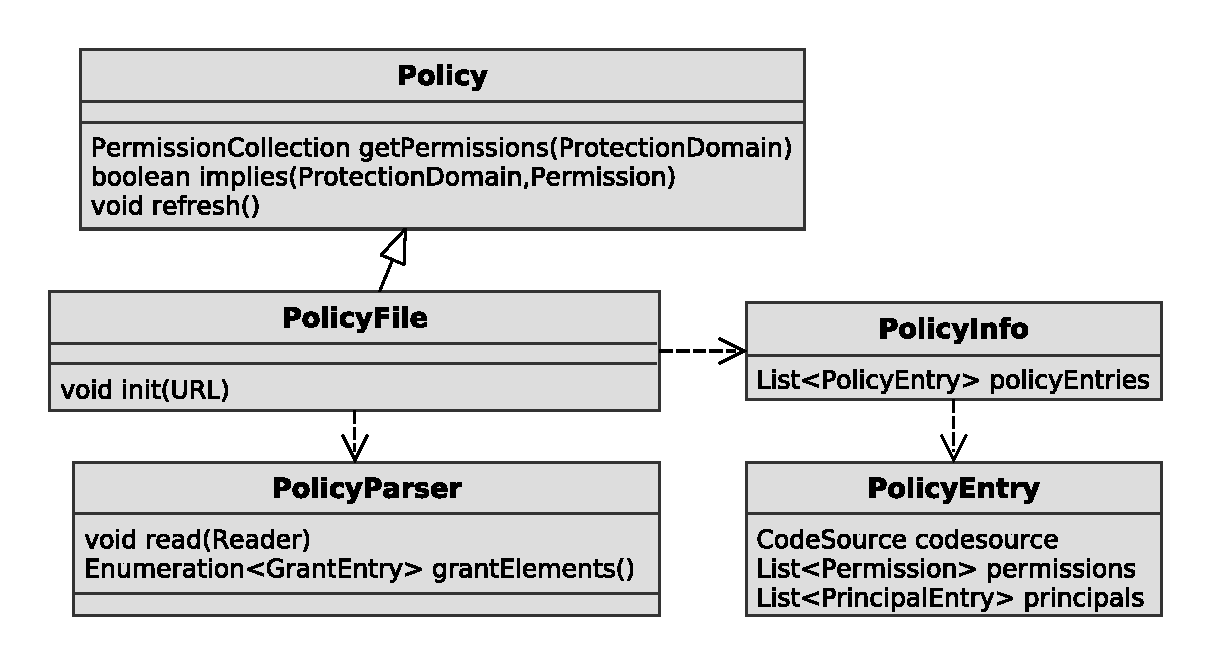
\includegraphics[width=12cm]{fig/policy-schema}
  \caption{Třídy podílející se na politice postavené na souboru politiky.}
  \label{tridyPolicyFile}
\end{figure}

Bezpečnostní politika používající soubory bezpečnostní politiky je realizována objektem třídy {\tt PolicyFile}.
Další třídy podílející se na zpracování souborů a uložení načtené bezpečnostní politiky v paměti ukazuje obrázek \ref{tridyPolicyFile}.

Objekt politiky {\tt PolicyFile} provádí rozhodnutí o oprávněnosti operací na základě aktuálního objektu {\tt PolicyInfo}.
Tento objekt obsahuje množinu položek bezpečnostní politiky, {\tt PolicyEntry}.

Protože tato množina je v průběhu načítání souborů bezpečnostní politiky tvořena postupně, je umístěna v tomto samostatném objektu.
Díky tomu je bezpečnostní politika vyměňována atomicky -- jeden objekt {\tt PolicyInfo} je v rámci atomické reference jen nahrazen novým.
V průběhu výměny bezpečnostní politiky tak nemůže dojít k okamžiku, kdy by byla uplatňována jen z části načtená politika.

K inicializaci a tedy i k načítání politiky ze souborů dochází při vytváření objektu {\tt PolicyFile} a při volání jeho metody {\tt refresh()}.
V obou případech jsou soubory politiky určeny konfiguračními proměnnými ({\it property}) popsanými v kapitole \ref{nastaveniPolitiky}.

%,,,,,,,,,,,,,,,,,,,,,,,,,,,,,,,,,,,,,,,,,,,,,,,,,,,,,,,,,,,,,,,,,,,,,,,,,,,,,
\subsubsection{Příklad souboru bezpečnostní politiky}
%'''''''''''''''''''''''''''''''''''''''''''''''''''''''''''''''''''''''''''''

Tento příklad ukazuje jednoduchou bezpečnostní politiku, opět v kontextu příkladu knihovny pro přístup k databázi z kapitoly \ref{databazeVsouboru}.

\begin{lstlisting}[caption=Příklad souboru bezpečnostní politiky, label=prikladSouboruBP]
grant codeBase "file:/srv/program/" {
  permission ZaznamPermission "Lucka", "nacteni";
};
grant codeBase "file:/srv/knihovna/" {
  permission ZaznamPermission "*", "nacteni";
  permission java.io.FilePermission "/srv/knihovna/data/-","read,write";
};
\end{lstlisting}

Program zde má přiděleno oprávnění k načtení záznamu \uv{Lucka}, nemůže ale přistupovat k s samotným databázovým souborů. K těm má oprávnění přistupovat jen knihovna zpřístupňující tuto databázi. Kvůli způsobu implementace kontroly oprávnění systémem řízení přístupu (popsaným v kapitole \ref{implementaceAC}) je nezbytné přidělit knihovně oprávnění ke všem záznamům v databázi, jinak by žádná kontrola oprávněnosti požadavku nemohla skončit pozitivně.

%,,,,,,,,,,,,,,,,,,,,,,,,,,,,,,,,,,,,,,,,,,,,,,,,,,,,,,,,,,,,,,,,,,,,,,,,,,,,,
\subsubsection{Zástupné znaky}
%'''''''''''''''''''''''''''''''''''''''''''''''''''''''''''''''''''''''''''''

URL kořene systému balíčků může být ukončeno zástupnými znaky pomlčka ({\tt -}) a hvězdička ({\tt *}).

Zatímco {\tt /*} odpovídá všem souborům v daném adresáři, {\tt /-} odpovídá všem souborům v daném adresáři i jeho podadresářích, rekurzivně.
V obou případech jsou zahrnuty jak soubory tříd ({\tt .class}), tak i celé archivy tříd ({\tt .jar}/{\tt .war}/{\tt .ear}).
Archivy vnořené v těchto archivech však již prohledávány nejsou.
\cite{jdkdocPolicyFiles}

%-----------------------------------------------------------------------------
\subsection{Nastavení třídy a souboru bezpečnostní politiky} \label{nastaveniPolitiky}
%-----------------------------------------------------------------------------

Tato kapitola popisuje nastavení implicitní třídy a souborů bezpečnostní politiky. Změna těchto nastavení dovoluje správci počítače
stanovit bezpečnostní politiku aplikovanou implicitně na všechny programy v Javě běžící na daném počítači.

Používaná třída a soubory bezpečnostní politiky jsou určeny globálně, pro celé běhové prostředí Javy (JRE -- Java Runtime Environment),
v konfiguračním souboru {\tt java.security} umístěném v podadresáři {\tt lib/security} adresáře JRE. \cite{refPolicyFiles}

Třída bezpečnostní politiky je určena svým celým jménem (např. {\tt sun.security.provider{\linebreak}.PolicyFile}) v konfigurační proměnné {\tt policy.provider}. \cite{refPolicyFiles}

Soubory bezpečnostní politiky jsou určeny svou absolutní adresou, uvedenou včetně protokolu (pro lokální soubory {\tt file:}),
v konfiguračních proměnných {\tt policy.url.n}, kde {\tt n} je pořadové číslo souboru. \cite{refPolicyFiles}

Načítání souborů bezpečnostní politiky začíná od {\tt policy.url.1} a postupně se {\tt n} inkrementuje a načítají se jednotlivé soubory bezpečnostní politiky,
dokud {\tt policy.url.n} existuje. \cite{refPolicyFiles}

\begin{lstlisting}[caption=Význačnější proměnné konfiguračního souboru {\tt java.security}, label=javasecurityexample]
policy.provider=sun.security.provider.PolicyFile
policy.url.1=file:${java.home}/lib/security/java.policy
policy.url.2=file:${user.home}/.java.policy
policy.url.3=file:/my-policies/my.policy
\end{lstlisting}

Příklady nastavení konfiguračních proměnných v tomto souboru jsou uvedeny v ukázce kódu \ref{javasecurityexample}, která je rozšířením příkladu z knihy pana Oakse. \cite[5.3.1]{oaks}

Nastavenou třídou bezpečnostní politiky je zde třída {\tt PolicyFile} a jako soubory bezpečnostní politiky jsou použity
soubory {\tt \$\{java.home\}/lib/security/java.policy}, {\tt \$\{user{\linebreak}.home\}/.java.policy} a {\tt /my-policies/my.policy} v uvedeném pořadí.

Implicitně jsou používány právě první dvě uvedená umístění -- {\tt \$\{java.home\}/lib/secu{\linebreak}rity/java.policy} pro celý systém a {\tt \$\{user.home\}/.java.policy} jako jeho rozšíření pro jednotlivé uživatele. Poslední umístění je přidáno pro demonstraci, jak je možné přidat další umístění. \cite{refSecurity}

Bezpečnostní politiku je dále možné rozšířit při startu JVM o další soubor bezpečnostní politiky. Stačí nastavit konfigurační proměnnou {\tt java.security.policy} při startu JVM: \cite[5.3.1]{oaks}

\begin{lstlisting}[caption=Spuštění JVM s vlastním souborem bezpečnostní politiky, label=nastaveniBP]
java -Djava.security.policy=dalsi_soubor_politiky.policy ProgramABC
\end{lstlisting}

V tomto případě bude uvedený soubor bezpečnostní politiky použit zároveň s výše uvedeným standardním souborem bezpečnostní politiky. Chceme-li standardní soubory bezpečnostní politiky určené souborem {\tt java.security} zcela nahradit, stačí namísto jednoho rovnítka v definici konfigurační proměnné použít rovnítka dvě: \cite[5.3.1]{oaks}

\begin{lstlisting}[caption=Spuštění JVM jen s vlastním souborem bezpečnostní politiky, label=nastaveniBP2]
java -Djava.security.policy==jediny_soubor_politiky.policy ProgramABC
\end{lstlisting}

Obsah této proměnné je možné změnit i za běhu programu, má-li daná část programu oprávnění k zápisu do této proměnné.

\begin{lstlisting}[caption=Nastavení souboru bezpečnostní politiky zevnitř JVM, label=nastaveniBP3]
System.setProperty("java.security.policy", "jiny_soubor_politky.policy");
\end{lstlisting}

Protože, jak již bylo zmíněno v kapitole \ref{souboryBP}, nové načtení bezpečnostní politiky ze souborů bezpečnostní politiky je možné provést
skrze metodu {\tt refresh()} objektu bezpečnostní politiky, je možné provedenou změnu bezpečnostní politiky nechat projevit jejím zavoláním:

\begin{lstlisting}[caption=Znovunačtení souboru bezpečnostní politiky, label=refreshBP]
Policy.getPolicy().refresh();
\end{lstlisting}

Problémem je, že tato metoda je označena jako nedoporučovaná ({\it deprecated}), protože je implementačně závislá -- zatímco u třídy bezpečnostní politiky {\tt PolicyFile} správně způsobí projevení změn v souboru bezpečnostní politiky, u jiných implementací bezpečnostní politiky může být implementována jako prázdná operace. \cite{refPolicy}

Tato práce se proto bude zabývat jen bezpečnostními politikami poskytovanými standardní implementací třídy {\tt Policy}, {\tt sun.security.provider.PolicyFile}, a na ní postavených nebo na ni delegujících implementacích.

%-----------------------------------------------------------------------------
\subsection{Statická a dynamická oprávnění ochranných domén} \label{staticPerm}
%-----------------------------------------------------------------------------

Oprávnění ochranných domén ({\tt ProtectionDomain}) popsaných v kapitole \ref{codeSourceAprotectionDomains} jsou ukládány přímo v objektech těchto ochranných domén,
konkrétně v jejich atributu {\tt permissions}. \cite{sourceProtectionDomain}

Protože jsou tato oprávnění do ochranné domény ukládány při jejím vytváření, tedy při zavádění třídy a následně nemohou být změněna, označujeme je jako statická.

Ochranné domény však souběžně mohou používat ještě oprávnění dynamická. Není-li ochranná doména označena jako používající výhradně statická oprávnění,
dotazuje se ochranná doména na oprávnění objektu bezpečnostní politiky při každém volání její metody {\tt implies()}.
Takto získaná oprávnění pak označujeme jako dynamická. \cite{sourceProtectionDomain}

Jsou-li dynamická oprávnění použita, efektivní oprávnění uplatňovaná metodou {\tt implies()} budou sjednocením dynamických a statických oprávnění třídy.
\cite{sourceProtectionDomain}

V současnosti jsou obvykle preferována oprávnění dynamická, jež poskytují vyšší variabilitu tím, že je možné bezpečnostní politiku vyměňovat za běhu
programu -- změny v ní se projeví jakmile začne být uplatňována metodou {\tt implies()} objektu bezpečnostní politiky, tedy zpravidla po volání metody
{\tt refresh()} používaného objektu bezpečnostní politiky.

Dynamická oprávnění jsou používána na všechny třídy zaváděné zavaděčem tříd z URL (viz \ref{URLClassLoader}) a jsou tedy využívána ve většině programů v Javě.
\cite{sourceURLClassLoader}

Umožňují navíc přidělovat oprávnění nejen na základě zdroje kódu, ale také na základě rolí uživatele spouštějícího daný kód. Tato dvě kritéria se však
obvykle používají pouze samostatně -- buď systém řízení přístupu ověřuje oprávnění kódu provést požadovanou operaci, nebo uživatelský kód ověřuje oprávnění
uživatele, který jej spouští, k provedení požadované operace. V obou případech se však stále jedná o dynamická oprávnění.

Statická oprávnění byla v Javě donedávna implementována jen v zájmu zachování kompatibility s verzemi Javy staršími než Java 2 SE 1.4. \cite{sourceProtectionDomain}
V současnosti se však statická oprávnění opět začaly používat a to za účelem optimalizace.

Získáváním oprávnění třídy z objektu bezpečnostní politiky pouze při zavádění třídy a ne při každém požadavku o ověření oprávněnosti k provedení operace je totiž možné proces ověřování oprávněnosti urychlit.

Zmíněná optimalizace se používá v rámci současných verzí aplikačního serveru WildFly pro ochranné domény tříd modulů aplikačního serveru, včetně uživatelských aplikací. Související problémy a jejich řešení jsou rozebrány v kapitole \ref{moduleClassLoader}.

%=============================================================================
\section{Celkový pohled na bezpečnost v Javě}
%=============================================================================

\begin{figure}[ht]
  \centering
  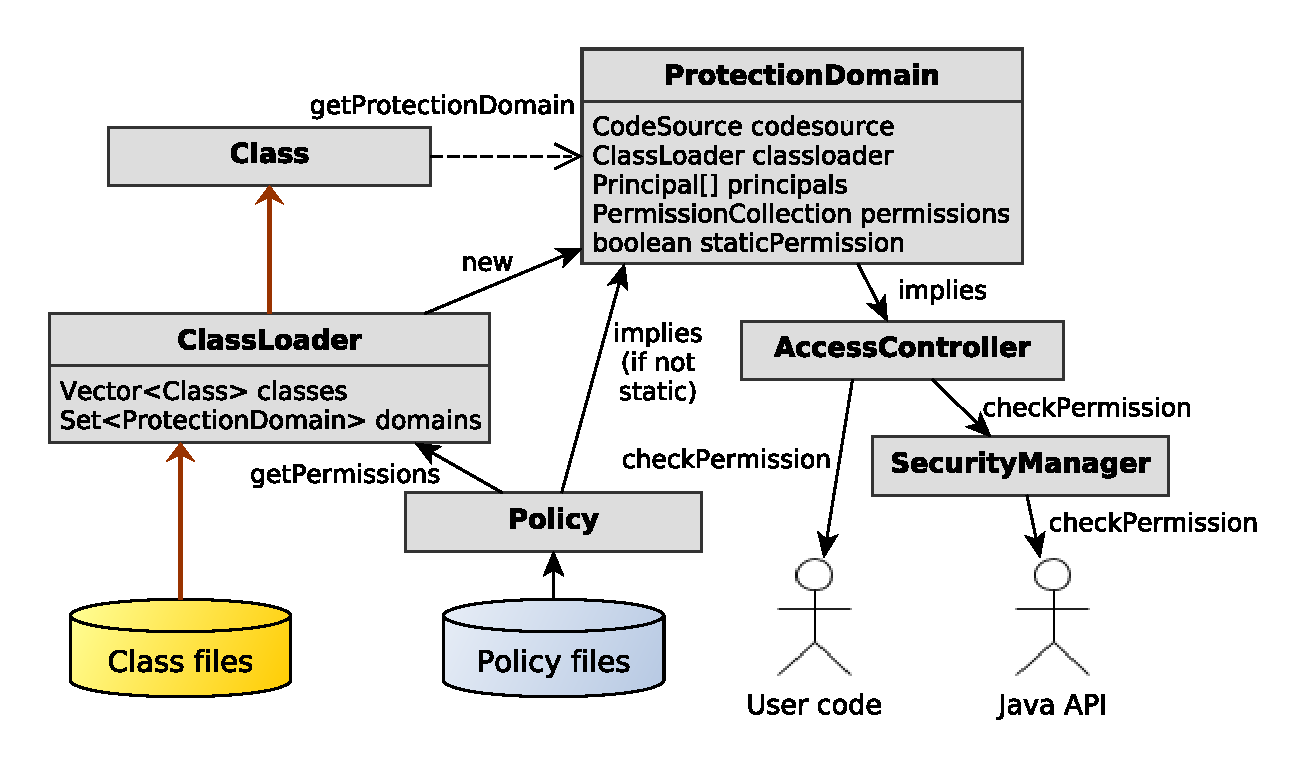
\includegraphics[width=14cm]{fig/domain-schema}
  \caption{Diagram datových toků tříd (hnědé šipky) a oprávnění tříd (černé šipky) v Javě}
  \label{diagramDatovychToku}
\end{figure}

Diagram datových toků na obrázku \ref{diagramDatovychToku} ukazuje putování informace o oprávněních třídy ze souboru bezpečnostní politiky až do systému řízení přístupu a správci bezpečnosti. Souvislé černé šipky představují přenos informace o oprávněních, zatímco hnědé přenos informace o třídách. Přerušované šipky představují reference. Směr šipky pak vede z třídy objektu s referenční proměnnou do třídy referencovaného objektu.

Ochranné domény a tím i statická oprávnění třídy jsou třídám přidělovány při jejich zavádění. Objekty ochranných domén ({\tt ProtectionDomain}) vytváří zavaděč tříd a to na základě jejich zdroje kódu ({\tt CodeSource}). Na statická oprávnění, která má zdroji kódu (a tedy i vytvořené ochranné doméně) zavaděč přidělit, se dotazuje aktuálně používaného objektu bezpečnostní politiky ({\tt Policy}).

Výstupem zavaděče tříd pak je objekt třídy ({\tt java.lang.Class}), jež nese referenci na svoji ochrannou doménu, která je společná všem objektům se stejným zdrojem kódu.

Systém řízení přístupu ({\tt java.security.AccessController}) pak rozhoduje na základě oprávnění v ochranné doméně a není-li ochranná doména označena jako používající výhradě statická oprávnění, také na základě odpovědi objektu bezpečnostní politiky ({\tt Policy}).

Na systém řízení přístupu pak rozhodování deleguje také standardní správce bezpečnosti ({\tt java.lang.SecurityManager}).


%%%%%%%%%%%%%%%%%%%%%%%%%%%%%%%%%%%%%%%%%%%%%%%%%%%%%%%%%%%%%%%%%%%%%%%%%%%%%%
\chapter{Distribuované prostředí Red Hat JBoss} \label{jboss}
%%%%%%%%%%%%%%%%%%%%%%%%%%%%%%%%%%%%%%%%%%%%%%%%%%%%%%%%%%%%%%%%%%%%%%%%%%%%%%

%=============================================================================
\section{Úvod do WildFly (JBoss AS)}
%=============================================================================

WildFly, dříve známý jako JBoss Application Server, je aplikační server standardu Java EE. Poskytuje běhové prostředí (nejen) Java EE aplikacím, které jsou na tomto aplikačním serveru nainstalovány. \cite{wildflyRename}

Jednotlivé instalace WildFly nazýváme hostiteli ({\it host}). Hostitel typicky odpovídá jednomu fyzickému serveru. V rámci každého hostitele může běžet více aplikačních serverů ({\it server}).
Hostitelé mohou být spojováni do domén ({\it domain}), přičemž jeden z nich v takovém případě zastává roli tzv. doménového řadiče ({\it domain controller}),
ke kterému se ostatní hostitelé domény registrují a nechají se jím spravovat. \cite{jbossDomainSetup}

Na doménovém řadiči leží jediný používaný konfigurační soubor domény, {\tt domain.xml}. Tento soubor obsahuje konfiguraci skupin serverů a profilů serverů a tím také konfiguraci subsystémů používaných na aplikačních serverech domény. \cite{jbossDomainSetup}

Každý hostitel má vlastní konfigurační soubor {\tt host.xml}. Tento soubor určuje název hostitele, zda-li je tento hostitel doménovým řadičem a pokud není také adresu doménového řadiče, proti kterému se registruje do domény. Zde jsou definovány aplikační servery, které na daném hostiteli poběží, porty na kterých budou poskytovat své služby a skupiny do kterých budou servery patřit. \cite{jbossDomainSetup}

Distribuovaného prostředí je docíleno nasazováním aplikací ({\it deployment}) na celé skupiny serverů najednou. Požadavky směřované na aplikaci by potom
měly být rozprostírány mezi všechny servery domény pomocí zařízení zvaného {\tt load balancer}. Toto zařízení umožňuje skrýt celou doménu za jedinou IP adresu
a umožnit klientům přistupujícím k aplikaci přístup k nejméně vytíženému serveru disponujícímu danou aplikací. \cite{jbossLoadBalancing}

%=============================================================================
\section{Běh WildFly pod správcem bezpečnosti Javy}
%=============================================================================

Na první pohled se může zdát, že nakonfigurovat použití správce bezpečnosti na aplikační server WildFly je možné stejně jako na jakoukoli jinou aplikaci v Javě -- nastavením patřičných konfiguračních vlastností popsaných v kapitolách \ref{souborPolitiky} a \ref{securityManager} při startu JVM. To je nejjednodušeji možné zajistit parametrem {\tt -D} příkazu {\tt java}. Ve spouštěcím skriptu WildFly ({\tt standalone.sh} / {\tt domain.sh} / {\tt standalone.bat} / {\tt domain.bat}) je pro tyto potřeby používána proměnná {\tt JAVA\_OPTS}. Připojením parametrů na konec této proměnné bychom měli dosáhnout použití správce bezpečnosti a bezpečnostní politiky ve všech JVM aplikačního serveru: \cite{jbossSecurityManager}

\begin{lstlisting}[caption=Doplnění spouštěcího skriptu o použití správce bezpečnosti, label=wildflySeSM]
JAVA_OPTS="$JAVA_OPTS -Djava.security.manager"
JAVA_OPTS="$JAVA_OPTS -Djava.security.policy==directory/wildfly.policy"
\end{lstlisting}

Dále vytvoříme soubor jednoduché bezpečnostní politiky.
Jestliže budeme dále předpokládat, že cílem nasazení bezpečnostní politiky na server je omezení možností uživatelských aplikací, můžeme od jemného přidělování jen nejnezbytnějších oprávnění každé součásti WildFly ustoupit k přidělení všech oprávnění všem součástem aplikačního serveru. Uživatelské aplikace nyní ponecháme bez jakýchkoli oprávnění a vyzkoušíme účinky této bezpečnostní politiky (viz kód \ref{wildflyPolicy}).

\begin{lstlisting}[caption=První testovací soubor bezpečnostní politiky pro WildFly, label=wildflyPolicy]
grant codeBase "file:${jboss.home.dir}/jboss-modules.jar" {
    permission java.security.AllPermission;
};
\end{lstlisting}

S použitím této bezpečnostní politiky se server WildFly skutečně bez potíží spustí. Když však na tento server nasadíme aplikaci provádějící kupříkladu čtení souboru uloženého v adresáři této aplikace, zjistíme že aplikace nemá problém tento soubor číst. Do souboru ležícího mimo jeho adresář se ale naopak nedostane, dokonce ani pokud toto oprávnění benevolentně přidělíme všem programům v JVM bez ohledu na jejich kořen balíčků ({\tt codeBase}).

Protože, použijeme-li naopak prázdný soubor bezpečnostní politiky, start serveru se nezdaří, je očividné že bezpečnostní politika byla nastavena správným způsobem, ale po startu aplikačního serveru byla aplikačním serverem dále ignorována.

Krokováním programu byly nalezeny dvě překážky, jež způsobovaly neúčinost bezpečnostní politiky ze souboru bezpečnostní politiky. Obě jsou popsány v následujících kapitolách.

%=============================================================================
\section{Správce bezpečnosti WildFly}
%=============================================================================

První překážkou je správce bezpečnosti WildFly ({\tt WildFlySecurityManager}) -- správce bezpečnosti používaný ve WildFly za účelem maximální optimalizace rychlosti aplikačního serveru.

Správce bezpečnosti WildFly používá vláknově lokální proměnnou {\tt CHECKING} pro omezení působnosti správce bezpečnosti. Je-li hodnota této proměnné referencí na objekt {\tt Boolean.TRUE}, jsou bezpečnostní kontroly akcí kontrolovaných správcem bezpečnosti prováděny. Jinak prováděny nejsou a kód pak běží stejně jako by správce bezpečnosti nebyl použit. \cite{sourceWildFlySecurityManager} (Dále v této kapitole bude používáno vyjádření, že správce bezpečnosti běží se zapnutými nebo s vypnutými kontrolami.)

Všechna vlákna WildFly pak implicitně běží se správcem bezpečnosti s vypnutými kontrolami. Kontroly by měly být zapnuty před zahájením provádění uživatelského kódu a opět vypnuty po jeho opuštění. \cite{sourceWildFlySecurityManager}

Toto je zvně správce bezpečnosti WildFly možné provést za pomoci metody {\tt WildFlySecurityManager.doChecked()}, jež zapne bezpečnostní kontroly správce bezpečnosti, provede kód jež jí je předán a následně bezpečnostní kontroly opět vypne. Zapnutí i vypnutí kontrol je přitom přeskočeno, byly-li už kontroly v době volání metody zapnuté, čímž je předejito problémům při vnořeném volání této metody. \cite{sourceWildFlySecurityManager}

Problémem však byla absence použití této metody při volání uživatelského kódu vyřizujícího HTTP požadavky. Tento problém jsem vzhledem k jeho rozsahu dočasně, pro potřeby řešení této práce, vyřešil vytvořením záplaty:

\begin{lstlisting}[caption=Záplata správce bezpečnosti WildFly nastavující bezpečnostní kontroly na implicitně zapnuté, label=patchSM]
-    private static final InheritableThreadLocal<Boolean> CHECKING
                 = new InheritableThreadLocal<>();
+    private static final InheritableThreadLocal<Boolean> CHECKING
                 = new InheritableThreadLocal<Boolean>(){
+        protected Boolean initialValue(){
+            return TRUE;
+        }
+    };
\end{lstlisting}

Tato záplata zajišťuje inicializaci proměnné {\tt CHECKING} na hodnotu {\tt TRUE}. Tato proměnná je vláknově lokální, každé vlákno má tedy její hodnotu uloženou zvlášť, přestože se jedná o vlastnost jednoho objektu. Navíc je tato vláknově lokální proměnná dědičná -- to znamená, že při vytvoření nového vlákna dědí toto vlákno hodnotu této proměnné svého rodičovského vlákna. \cite{refInheritableThreadLocal}\cite{refThreadLocal}

Hodnota proměnné je inicializována při prvním pokusu o získání její hodnoty metodou {\tt get()}, nebyla-li dříve nastavena voláním metody {\tt set()}. Hodnota na kterou je proměnná incializována je určena voláním metody svého objektu, {\tt initialValue()}. Tato metoda vrací implicitně {\tt null}. Jiné implicitní hodnoty lze dosáhnout přepsáním této metody vlastní implementací. Právě přepisem této metody je stanovena i implicitní hodnota proměnné {\tt CHECKING} v mé záplatě na {\tt TRUE} (Kód \ref{patchSM}). \cite{refThreadLocal}

Tato záplata ale zapíná bezpečnostní kontroly pro celou JVM -- popírá tak původní smysl správce bezpečnosti Wildfly, kterým měla být maximální rychlostní optimalizace aplikačního serveru, na což jsem byl také upozorněn při žádosti o začlenění mé záplaty do vývojové verze WildFly Security Manageru jeho vývojáři. \cite{smPullRequest}

Pravděpodobně protože hledání trvalého a koncepčního řešení trvalo již skoro půl roku, byla nakonec, i přes její nekoncepčnost, mnou navržená změna začleněna. \cite{smPullRequest}\cite{smPullRequestImpl}

Další změnou provedenou ve správci bezpečnosti WildFly pro potřeby řešení této práce bylo povolení změny správce bezpečnosti. Tato změna byla nezbytná pro vypínání správce bezpečnosti ze subsystému navrhovaného a popsaného v následujících kapitolách.

\begin{lstlisting}[caption=Záplata správce bezpečnosti WildFly umožňující vypnutí správce bezpečnosti (zkráceno), label=patchSM]
     public void checkPermission(Permission perm, AccessControlContext context) {
         if (perm.implies(SECURITY_MANAGER_PERMISSION)) {
-            throw access.secMgrChange();
+            //throw access.secMgrChange();
         }
\end{lstlisting}

Jak je vidět, spočívá v prostém zakomentování tohoto omezení v metodě správce bezpečnosti ověřujícího povolení prováděné operace -- {\tt checkPermission()}. Toto omezení sice posiluje bezpečnost systému, avšak oslabuje schopnosti bezpečnostních politik, které tak ztrácí možnost povolit uživatelskému kódu (nebo i kódu modulů WildFly) změnu správce bezpečnosti.

Posílení bezpečnosti navíc není až tak výrazné, považujeme-li kód modulů WildFly za důvěryhodný -- uživatelskému kódu ve výměně správce bezpečnosti nadále brání samotná bezpečnostní politika, není-li její součástí výslovné povolení změny správce bezpečnosti.

%=============================================================================
\section{Zavaděč tříd modulů WildFly} \label{moduleClassLoader}
%=============================================================================

Protože se překonáním problému se správcem bezpečnosti WildFly popsaném v předchozí kapitole problém neúčinosti souborů bezpečnostní politiky nevyřešil,
pokračoval jsem ve snahách o nalezení zdroje tohoto problému.

Krokováním programu se podařilo ověřit, že používaný objekt bezpečnostní politiky úspěšně opouští správná sada oprávnění. Problém tedy není v žádném
z objektů bezpečnostní politiky které jsou ve WildFly používány. Volání metod {\tt implies()} i {\tt getPermissions()} ochranné domény však vracelo výsledek,
který byl od této sady zcela odlišný.

První problém tak spočíval v oprávněních ukládaných do objektu ochranné domény. Průzkum kódu zavaděče tříd používaného ve WildFly odhalil příčinu:
Zavaděč tříd modulů WildFly ({\tt org.jboss.modules.ModuleClassLoader}) implicitně zcela ignoruje oprávnění poskytovaná objektem bezpečnostní politiky.

Tento problém bylo možné vyřešit celkem snadno -- zavaděč umožňoval nastavit používání bezpečnostní politiky ze souboru nastavením k tomu určené
konfigurační vlastnosti. Aby tedy začaly být bezpečnostní politiky uplatňovány, stačí přidat její definici do spouštěcího skriptu WildFly: \cite{sourceModuleClassLoader}

\begin{lstlisting}[caption=Úprava spouštěcího skriptu pro spuštění se souborem bezpečnostní politiky, label=jbossOpts]
JAVA_OPTS="$JAVA_OPTS -Djboss.modules.policy-permissions=true"
JAVA_OPTS="$JAVA_OPTS -Djava.security.manager"
JAVA_OPTS="$JAVA_OPTS -Djava.security.policy==directory/wildfly.policy"
\end{lstlisting}

Po spuštění aplikačního serveru v této konfiguraci již jsou uplatňovány bezpečnostní politiky. Pokud se však pokusíme změnit je za běhu aplikace,
například za pomoci řešení implementovaného v kapitole \ref{implementace}, výměna politiky se na třídách, které už byly načteny do paměti, neprojeví.

Důvodem je, že i přesto, že nyní již jsou třídám zavaděčem přidělovány oprávnění z objektu bezpečnostní politiky, tyto oprávnění jsou přidělovány
jako statická, tedy jen při načítání třídy.

V rámci této práce byla tedy vytvořena záplata zavaděče tříd modulů WildFly, která umožní používání oprávnění z objektu bezpečnostní politiky
ve formě dynamických oprávnění ochranné domény.

\begin{lstlisting}[caption=Hlavní část záplaty umožňující nastavit používání dynamických oprávnění, label=refreshable]
+  if (POLICY_REFRESHABLE) {
+      protectionDomain = new ProtectionDomain(codeSource, permissions,
+                                 this, null); // staticPermission=false
+  }else if (POLICY_PERMISSIONS && POLICY_READY.get()) {
-  if (POLICY_PERMISSIONS && POLICY_READY.get()) {
\end{lstlisting}

V předchozí variantě byla do ochranné domény ukládána množina oprávnění odpovídající sjednocení oprávnění z objektu bezpečnostní politiky a oprávnění modulu, udělená specifikací Java EE nebo konfiguračním souborem {\tt permission.xml}.

V nové variantě stačí do ochranné domény uložit oprávnění modulu a nastavit ochrannou doménu jako používající dynamická oprávnění - uvést třetí a čtvrtý parametr konstruktoru. Použití záplatou vytvořené varianty je podmíněno nastavením nové konfigurační vlastnosti {\tt jboss.modules.policy-refreshable} na hodnotu {\tt true}.

%%%%%%%%%%%%%%%%%%%%%%%%%%%%%%%%%%%%%%%%%%%%%%%%%%%%%%%%%%%%%%%%%%%%%%%%%%%%%%
\chapter{Návrh systému} \label{navrh}
%%%%%%%%%%%%%%%%%%%%%%%%%%%%%%%%%%%%%%%%%%%%%%%%%%%%%%%%%%%%%%%%%%%%%%%%%%%%%%

Cílem práce je vytvoření systému pro centralizovanou správu a distribuci bezpečnostních politik. Měl by umožnit nasazovat bezpečnostní politiky na jednotlivé servery domény WildFly a sledovat také, které bezpečnostní politiky jsou právě na kterých serverech domény WildFly nasazeny.

Jako příhodné se pro tento účel zdá využití rozšiřitelnosti systému WildFly a implementace zmíněné funkcionality formou subsystému aplikačního serveru WildFly. Subsystém je rozšířením aplikačního serveru a jeho konfigurace i přítomnost je nastavována zvlášť pro každý profil, přičemž profil je souhrnem konfigurace serveru a je nastavovaný pro celé skupiny serverů. Optimálním řešením by bylo takové rozšíření WildFly, jež by bylo nasazováno a konfigurováno nezávisle na profilech jednotlivých serverů. Takový koncept ale bohužel WildFly neposkytuje.

Nadále proto budeme předpokládat, že všechny skupiny serverů, v rámci kterých chceme s bezpečnostními politikami manipulovat, používají stejný konfigurační profil.

%=============================================================================
\section{Způsob nastavení bezpečnostní politiky}
%=============================================================================

Uživatel i aplikace mohou se subsystémem komunikovat prostřednictvím JBoss native management API. To je navrženo pro maximální jednoduchost a k nejrůznějším nastavením, které by jinak byly reprezentovány objekty velkého množství tříd, je možné přistupovat jako ke stromu objektů obecných tříd uzel ({\tt ModelNode}) a vlastnost (Property). Uzly tvoří strom a každý uzel může mít vlastnosti, jež obsahují samotnou konfiguraci aplikačního serveru ve formě textových řetězců ({\tt String}), do kterých tedy musí být převedeny i hodnoty jiných datových typů. \cite{jbossDetypedManagement}

Klient JBoss native management API, kterým jsou zejména CLI rozhraní WildFly a Webová konzola WildFly, tedy musí implementovat jen práci s tímto konfiguračním stromem. Jeho implementace tedy teoreticky nemusí vůbec záviset na typu informace v konfiguračním stromu. V praxi toto ale pochopitelně platí jen pro nízkoúrovňové nástroje sloužící k přímé úpravě konfiguračního stromu, jakým je CLI rozhraní WildFly. Webová konzola naproti tomu pracuje s více konkrétními třídami objektů, jakými jsou server, skupina ({\tt server-group}) nebo zdroj dat ({\tt datasource}). Přestože pracuje se stejným konfiguračním stromem, tvořeným jen těmito dvěma datovými typy, je závislá na struktuře kterou uzly tohoto stromu tvoří. Jednoduchost JBoss native management API je tak znatelná spíše jen na stabilitě tohoto API a knihovně pro práci s ním -- {\tt jboss-dmr}. \cite{jbossDetypedManagement}

Rozšíření aplikačního serveru, kterým je například subsystém, vykonává svůj kód zejména v reakci na události, které si zaregistruje. Těmito událostmi bývá zpravidla načtení rozšíření a přidání a odebrání subsystému, často také operace nad uživatelským balíčkem (nasazení apod.) nebo právě operace nad definovanou konfigurační vlastností. \cite{WildFlyExtending}

Jako vhodné řešení bylo tedy zvoleno nasazení bezpečnostní politiky v návaznosti na nastavení hodnoty konfigurační proměnné. Každý server aplikačního serveru bude mít v konfiguračním stromu svůj uzel a jeho vlastnostmi bude bude určen soubor bezpečnostní politiky, jež by měl být nasazený na daném serveru a také to, zda by měl být security manager pro daný server vůbec zapnutý.

Samotná operace provedení výměny bezpečnostní politiky a případného zapnutí/vypnutí security manageru pak bude spojena s událostí nastavení hodnoty dané vlastnosti. Vlastnosti bude přiřazena metoda, jež má být volána při zápisu do její hodnoty. Ta zajistí výměnu bezpečnostní politiky prostřednictvím k tomu určené třídy, jež bude součástí vytvářeného subsystému.

%=============================================================================
\section{Způsob šíření souborů bezpečnostní politiky} \label{sireniSouboru}
%=============================================================================

Jelikož cílem práce není jen centralizovaná správa, ale i distribuce bezpečnostních politik, je nutné rovněž stanovit způsob, jakým soubory bezpečnostní politiky budou šířeny mezi servery WildFly domény.

Jako pravděpodobně nejjednodušší řešení, které by bylo možné navrhnout, lze označit vytvoření sdíleného adresáře, jež by byl přístupný z každého serveru domény, například protokolem NFS (Network File System).

S tímto řešením však souvisí hned několik potíží. První z nich je vyšší platformní závislost -- zatímco WildFly jakožto aplikace v Javě bez problému běží na mnoha platformách a pod různými operačními systémy, protokol NFS není napříč operačními systémy příliš podporován. Tento problém by bylo možné řešit použitím více rozšířeného protokolu umožňujícího vzdálený přístup k souborům, jakým je například FTP.

Druhým problém je ale bezpečnost -- protokoly FTP ani NFS samy o sobě nedokáží zaručit autenticitu serveru, ke kterému se klient připojuje. Případný útočník by se tak mohl vydávat za FTP/NFS server na němž jsou bezpečnostní politiky uložené a podvrhnout tak serverům domény vlastní bezpečnostní politiky. Tento problém by mohlo vyřešit použití lépe zabezpečeného protokolu, jakým je například SSH (Secure Shell), jež umožňuje vzdálený přístup k souborům prostřednictvím SSHFS (SSH Filesystem), nebo FTPS (FTP over SSL), kde se server vůči klientovi autentizuje za pomoci asymetrické kryptografie. \cite[3]{ssh}

Použití těchto lépe zabezpečených protokolů zajistí bezpečnost systému, avšak umocní problém platformních omezení, obzvláště v případě protokolu SSH. Navíc i v případě dokonalého zajištění sdíleného adresáře bezpečnostních politik bude nutné zajistit také bezpečný přenos informací po JBoss Native API, pro bezpečný přenos informace, kterou bezpečnostní politiku má daný server použít.

Problém bezpečnosti distribuce bezpečnostních politik je možné si představit jako řetěz. Řetěz je jen tak silný, jak silný je jeho nejslabší článek. Aby byl řetěz silný, je třeba mít silné všechny jeho články -- v tomto případě bezpečnost komunikačního kanálu, po kterém se přenáší soubory bezpečnostních politik a komunikačního kanálu, po kterém se přenáší informace, který soubor bezpečnostní politiky by měl daný server použít.

Touto úvahou lze dojít k závěru, že optimálním řešením je minimalizovat počet článků řetězu -- sloučit tyto dva komunikační kanály do jediného a nadále řešit bezpečnost jen tohoto jediného komunikačního kanálu.

Toto lze implementovat za pomoci uzlů konfiguračního stromu jednotlivých politik představujících jednotlivé soubory politik. Vlastností tohoto uzlu by pak obsah samotného souboru bezpečnostní politiky. Soubory bezpečnostní politiky by pak mohly být nahrávány do těchto vlastností konfiguračních uzlů na straně doménového řadiče a naopak z nich čteny na straně ostatních členských serverů WildFly domény.

Protože však použití standardní třídy bezpečnostní politiky ({\tt sun.security.provider.PolicyFile}) vyžaduje soubory bezpečnostní politiky přístupné skrze URL adresu souboru, je na straně členských serverů třeba před aplikací bezpečnostní politiky obsah souboru bezpečnostní politiky zapsat do dočasného souboru.

Protože bude tento postup nezbytné aplikovat na straně členských serverů domény, je zbytečné řešit toto na doménovém řadiči jinak. Ztrácí se tak také většina důvodů pro to, aby byly bezpečnostní politiky na straně doménového řadiče uloženy v souboru souborového systému.

Jako výhodnějším řešením se tedy začíná jevit ukládat bezpečnostní politiky přímo do vlastností konfiguračních uzlů. Tím bude vyřešen i problém, jak ze strany aplikačního serveru detekovat, že byl soubor bezpečnostní politiky změněn. Zatímco v případě souboru by bylo nezbytné se periodicky dotazovat na čas poslední změny tohoto souboru, na změnu hodnoty konfigurační vlastnosti je možné navázat programovou událost, a tím zajistit aplikaci bezpečnostní politiky přímo v návaznosti na změnu hodnoty její konfigurační vlastnosti.

%=============================================================================
\section{Webové uživatelské rozhraní} \label{navrhGUI}
%=============================================================================

Součástí zadání práce bylo také vytvořit webové rozhraní pro komunikaci s uživatelem. Jelikož je samotné jádro řešení implementováno jako subsystém WildFly, jako optimální řešení se nabízelo implementovat uživatelské rozhraní tohoto subsystému jako rozšíření webové konzoly WildFly.

Webová konzola WildFly je standardní součástí aplikačního serveru WildFly. Je GWT aplikací běžící na straně klienta, ve webovém prohlížeči, a se serverem komunikuje prostřednictvím HTTP Management API. To je alternativou Native API -- plní stejnou funkci, ale běží nad protokolem HTTP. Tělem odpovědí serveru i tělem POST dotazů klienta je JSON reprezentace uzlu konfiguračního stromu ({\tt ModelNode}). \cite{WildFlyManagementAPIreference}

\begin{figure}[ht]
  \centering
  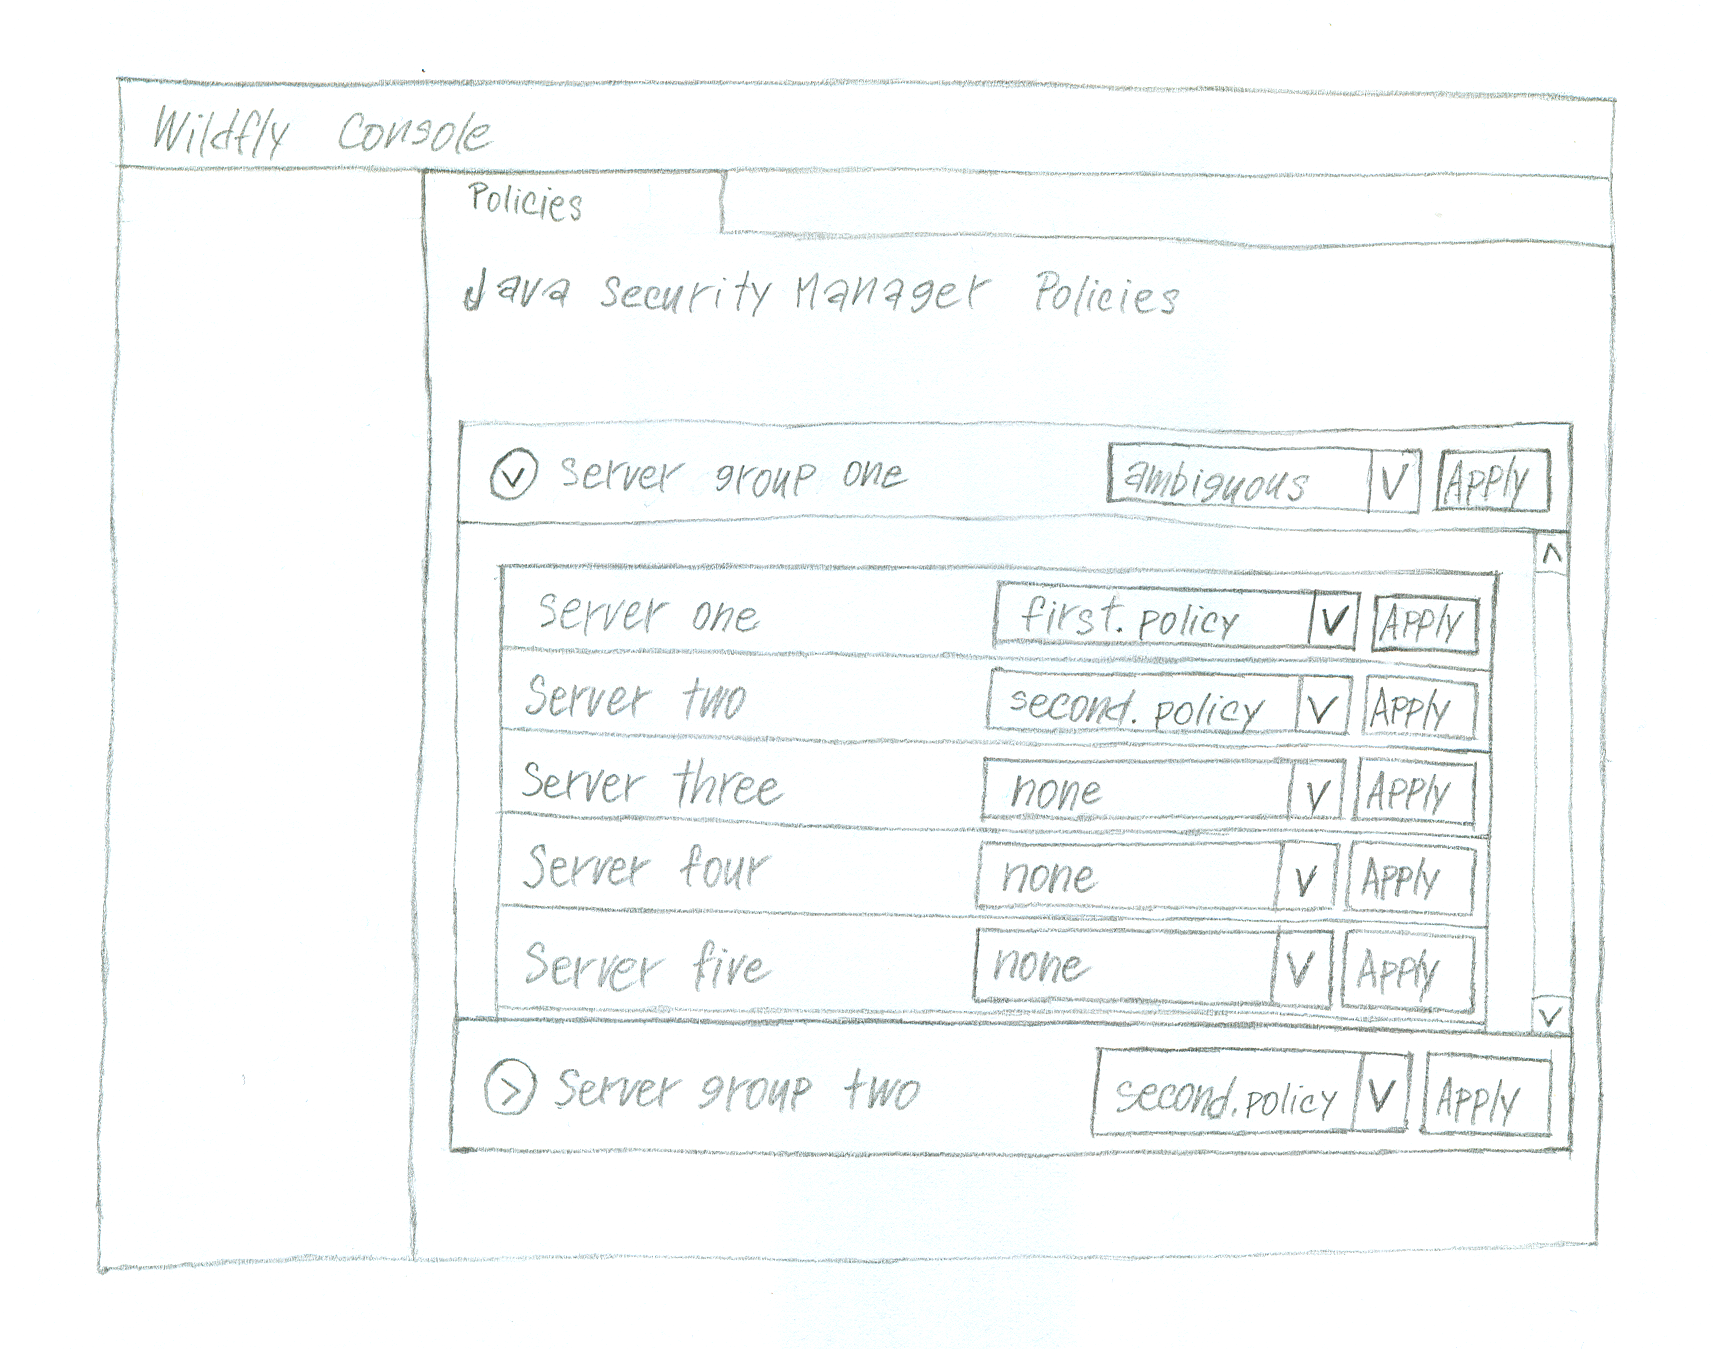
\includegraphics[width=14cm]{fig/mockup}
  \caption{Grafický návrh uživatelského rozhraní plánovaného rozšíření WildFly.}
\end{figure}

\begin{figure}[ht]
  \centering
  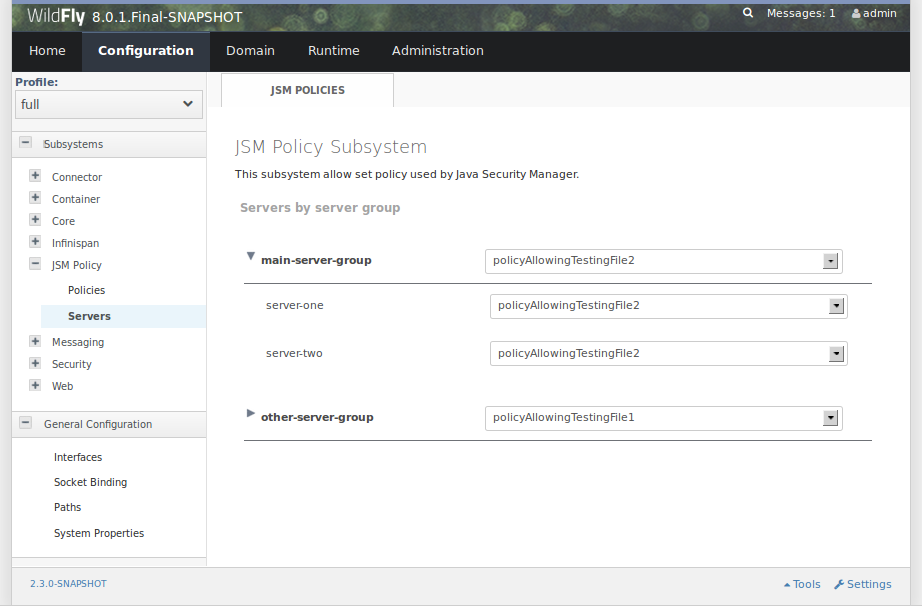
\includegraphics[width=14cm]{fig/jsmpolicy-servers}
  \caption{Výsledná podoba webového uživatelského rozhraní.}
\end{figure}

%%%%%%%%%%%%%%%%%%%%%%%%%%%%%%%%%%%%%%%%%%%%%%%%%%%%%%%%%%%%%%%%%%%%%%%%%%%%%%
\chapter{Popis implementace systému} \label{implementace}
%%%%%%%%%%%%%%%%%%%%%%%%%%%%%%%%%%%%%%%%%%%%%%%%%%%%%%%%%%%%%%%%%%%%%%%%%%%%%%

%=============================================================================
\section{První etapa}
%=============================================================================

V rámci první etapy implementace řešení byl implementován jednoduchý subsystém WildFly za pomoci kostry subsystému z Maven repozitáře, podle dokumentace WildFly 8 věnující se právě vytváření rozšíření WildFly. \cite{WildFlyExtending}

Dle tohoto vzoru byl vytvořen subsystém, jehož jedinou funkcí bylo rozšíření konfiguračního stromu o uzly {\tt server=*} uchovávající informaci o URL bezpečnostních politik, jež by měly být uloženy na jednotlivých serverech domény WildFly odpovídajících svým jménem jménu tohoto konfiguračního uzlu. Tyto uzly fungovaly jako běžné uzly konfiguračního stromu WildFly -- administrátor měl možnost je vytvářet, odstraňovat a nastavovat jejich vlastnost {\tt policy}, jež nesla právě samotnou URL nasazené bezpečnostní politiky.

Na změnu této konfigurační vlastnosti zároveň server domény daný jménem uzlu reagoval právě nasazením dané bezpečnostní politiky, prostřednicvím registrace této události při tvorbě konfigurační vlastnosti {\tt policy} uzlu {\tt server=*}.

Toho bylo dosaženo vytvořením třídy {\tt ServerWriteAttributeHandler} a jejím uvedením v rámci volání provádějícího registraci samotné konfigurační vlastnosti:

\begin{lstlisting}[caption=Registrace konfigurační vlastnosti {\tt policy} uzlu {\tt server=*}, label=registraceAtributu]
resourceRegistration.registerReadWriteAttribute(POLICY,
                null, ServerWriteAttributeHandler.INSTANCE);
\end{lstlisting}

Není stanovena třída zprostředkovávající čtení tohoto konfigurační vlastnosti. (Na jejím místě je uveden {\tt null}) Na čtení této vlastnosti není totiž vázána žádná akce, ani není nutné obsah vracený jako odpověď na pokus o čtení vlastnosti nikterak upravovat a je možné uživatele nechat číst samotnou vlastnost přímo.

Aby byla bezpečnostní politika aplikována nejen na základě akce administrátora, ale také automaticky po startu serveru, byla její aplikace navázána také na akci přidání nového uzlu {\tt server=*}. Odstranění takového uzlu pak bude navázáno na odebrání bezpečnostní politiky, stejně jako kdyby byla vlastnost {\tt policy} nastavena na nedefinovanou.

Obě akce je jsou implementovány jako třídy {\tt ServerAdd} a {\tt ServerRemove}, jež jsou na uzly typu {\tt server=*} navázány skrze parametry konstruktoru třídy definující tento uzel konfiguračního stromu:

\begin{lstlisting}[caption=Definice konfiguračního uzlu {\tt server=*}, label=registraceUzluServer]
public class ServerDefinition extends SimpleResourceDefinition {
    private ServerDefinition() {
        super(JsmPolicyExtension.SERVER_PATH,
                JsmPolicyExtension.getResourceDescriptionResolver("server"),
                ServerAdd.INSTANCE,
                ServerRemove.INSTANCE);
    }
}
\end{lstlisting}

Konfigurační uzly {\tt server=*} jsou ukládány do konfiguračního XML souboru domény WildFly, jak je u konfigurační uzlů WildFly běžné. Ukládání veškeré konfigurace subsystému je implementováno ve třídě {\tt SubsystemParser}.

%=============================================================================
\section{Druhá etapa}
%=============================================================================

V rámci druhé etapy bylo uživatelské rozhraní pozměněno dle grafického návrhu předvedeného v kapitole \ref{navrhGUI}. V souvislosti s touto změnou bylo nutné rozšířit rovněž subsystém WildFly. Jeho dosavadní implementace neumožňovala výběr bezpečnostní politiky formou výběru v rozbalovací nabídce.

Výběr formou rozbalovací nabídky vyžaduje od aplikace zobrazující nabídku znalost voleb, mezi nimiž může uživatel provádět výběr. To při dosavadní implementaci subsystému možné nebylo, neboť aplikace běžící na straně webového prohlížeče měla přístup k souborům (tedy i souborům bezpečnostních politik) možný jen právě prostřednictvím subsystému, který doposud přístup k seznamu souborů bezpečnostních politik neumožňoval.

Do konfiguračního stromu subsystému tak vedle dosavadních uzlů {\tt server=*} popsaných v minulé podkapitole přibyly uzly {\tt policy=*}, jež reprezentovaly právě jednotlivé soubory bezpečnostní politiky, jež bylo možné jako bezpečnostní politiky jednotlivých serverů nastavit. Tyto uzly nebyly ukládány do konfiguračního XML souboru aplikačního serveru, ale byly vytvářeny ze seznamu souborů nacházejících se v k tomu určeném adresáři aplikačního serveru.

Toto načítání seznamu souborů nebylo řešeno cestou ideální, za kterou by šlo nejspíše považovat přímé navázání jakéhokoli pokusu o čtení těchto konfiguračních uzlů na programovou obsluhu, jež by umožnila jako přímý výsledek tohoto dotazu vrátit přímo aktuální seznam souborů v adresáři bezpečnostních politik.

Vzhledem k ranosti této verze a odstranění těchto schopností systému v pozdějších etapách vývoje bylo načtení seznamu souborů bezpečnostních politik řešeno přímým vytvořením těchto konfiguračních uzlů při startu aplikačního serveru na základě obsahu adresáře bezpečnostních politik ve chvíli startu aplikačního serveru.

Hlavní nevýhodou tohoto přístupu byla přetrvávající potřeba zajištění přístupu k souborům bezpečnostních politik uložených na doménovém řadiči, nikoli však již na jednotlivých aplikačních serverech domény. Adresář bezpečnostních politik tak bylo nutné napříč aplikačními servery distribuovat jinou cestou. (Podrobněji popsanou v kapitole \ref{navrhGUI} zabývající se návrhem právě způsobu šíření souboru bezpečnostních politik.)

Později odhaleným nedostatkem se pak stal fakt, že do konfigurační vlastnosti {\tt policy} byla ukládána absolutní cesta k souboru bezpečnostní politiky, což by výrazně zkomplikovalo ostré nasazení implementovaného systému.

%=============================================================================
\section{Třetí etapa}
%=============================================================================

V rámci třetí etapy implementace byl subsystém WildFly upraven, aby konfigurační strom WildFly nefungoval jen jako úložiště adres nastavených bezpečnostních politik, ale také jako úložiště samotných bezpečnostních politik.

Byl tedy pozměněn význam konfigurační vlastnosti {\tt file} uzlu {\tt policy=*}. Absolutní URL adresa souboru  bezpečnostní politiky byla nahrazena obsahem souboru bezpečnostní politiky.

Zároveň byl změněn význam konfigurační vlastnosti {\tt policy} uzlu {\tt server=*}, jež doposud rovněž obsahoval URL adresu souboru bezpečnostní politiky nasazené na daném serveru. Nově byl nahrazen jménem uzlu {\tt policy=*}, jehož bezpečnostní politika z jeho vlastnosti {\tt file} byla na daný server nově nasazována.

Nadále tak nestačilo provádět aplikaci bezpečnostní politiky při změně atributu {\tt policy} uzlu {\tt server=*}, ale bylo nutné bezpečnostní politiku používanou aplikačním serverem vyměnit rovněž při změně obsahu vlastnosti {\tt file} uzlu {\tt policy=*}.

Toto je řešeno analogicky jako právě v případě akce navázané na změnu vlastnosti uzlu serveru -- vytvořením třídy {\tt PolicyWriteAttributeHandler} a jejím navázáním na vlastnost uzlu bezpečnostní politiky.

%%%%%%%%%%%%%%%%%%%%%%%%%%%%%%%%%%%%%%%%%%%%%%%%%%%%%%%%%%%%%%%%%%%%%%%%%%%%%%
\chapter{Testování systému} \label{testovani}
%%%%%%%%%%%%%%%%%%%%%%%%%%%%%%%%%%%%%%%%%%%%%%%%%%%%%%%%%%%%%%%%%%%%%%%%%%%%%%

Protože cílem této bakalářské práce nebylo jen vytvoření systému umožňujícího správu bezpečnostních politik nasazených na jednotlivých serverech distribuovaného systému ale také jeho otestování, tato kapitola se zabývá tvorbou testů, umožňujících otestovat implementované řešení.

Testování je nedílnou součástí vývoje software a je užíváno k odhalení vad software a prokázání, že software dosáhl požadované úrovně kvality v zadaných kritériích. Obvykle se provádí za pomoci automatizovaných programů, takzvaných testů. \cite{ivsTest}

Testy se běžně dělí následovně: \cite{testsTypes}\cite{ivsTest}

\begin{enumerate}
  
  \item {\textbf Jednotkové testy (Unit tests)} testují jednotlivé jednotky systému. Jednotkou je typicky třída programovacího jazyka. Každá jednotka se testuje samostatně, s maximální snahou o izolaci od ostatních součástí systému. Jejich cílem je především ověřit, zda jednotlivé jednotky splňují svoji specifikaci -- dodávají na základě testovacího vstupu odpovídající výstup. Nijak neřeší problémy v komunikaci jednotlivých jednotek mezi sebou nebo se zbytkem systému (v tomto případě aplikačním serverem WildFly). \cite{testsTypes}\cite{ivsTest}
  
  \item {\textbf Systémové testy (System tests)} testují celý systém jako jediný celek a umožňují ověřit zda systém jako celek dokáže plnit svůj účel, pro který byl vytvořen. Testovaný systém ovlivňují a kontrolují zpravidla z jeho vnějšku. \cite{testsTypes}\cite{ivsTest}
  
  \item {\textbf Integrační testy (Integration tests)} jsou mezistupněm mezi jednotkovými a systémovými testy. Jak jejich název napovídá, jejich hlavním účelem je ověřit zda spolu testované jednotky správně spolupracují. \cite{testsTypes}\cite{ivsTest}
  
\end{enumerate}

Protože lze systémové testy někdy chápat také jako zvláštní případ integračních testů, jsou systémové testy někdy mezi integrační testy zahrnovány. \cite{testsUnitVsInteg}

%=============================================================================
\section{Jednotkové testy}
%=============================================================================

Jednotkové testy tedy umožňují testovat jednotlivé jednotky systému a těmito jednotkami, po kterých se systém testuje, jsou typicky třídy programovacího jazyka. Každé třídě programu by v ideálním případě měla být přidělena jedna třída testu, jež by měla ověřit správnost fungování této třídy.

Testované jednotky by měly být testovány ve vzájemné izolaci. Toho se dosahuje buď jejich vhodným návrhem, nebo použitím napodobenin objektů ({\it mock object}) z jiných jednotek, na kterých tato jednotka závisí.

Komplikace jež by mohly ohrozit samotnou výměnu bezpečnostní politiky nebo správce bezpečnosti vyplývají převážně z integrace s aplikačním serverem WildFly. Vytvoření jednotkových testů pro výměnu bezpečnostní politiky a správce bezpečnosti by tedy nebylo příliš užitečné.

Byly však vytvořeny jednotkové testy pro testování podpůrných součástí implementovaného subsystému -- testy syntaktické kontroly souborů bezpečnostní politiky a práce s konfiguračním podstromem DMR subsystému.

%=============================================================================
\section{Integrační testy}
%=============================================================================

Integrační testy testují systém jako celek. Implementovaný systém byl tímto způsobem testován na schopnost plnění základních požadavků daných zadáním této práce -- schopnosti zapnout a vypnout správce bezpečnosti a vyměnit používanou bezpečnostní politiku skrze administrační protokol WildFly.

Byl tedy vytvořen integrační test umožňující otestovat zmíněné schopnosti na běžícím aplikačním serveru WildFly s nainstalovaným subsystémem pro nastavení bezpečnostní politiky, jehož vytvoření je popsáno v kapitole \ref{implementace}.

Tento test se skládá ze dvou částí -- agenta, aplikace nasazované na testovaný server, a manažeru -- testu vytvořeného za pomoci knihovny JUnit, řídícího proces samotného testování.

Agent je Java EE aplikací nabízející své služby skrze rozhraní REST. Službami, jež poskytuje, je zejména otestování schopnosti provést vybranou akci z pozice aplikace nasazené na testovaném serveru. Klient rozhraní REST se tedy k této službě může připojit a požádat o otestování schopnosti provést vybranou operaci. Jako odpověď pak dostane informaci, zda-li se provedení této operace zdařilo, nebo zda bylo zmařeno Access controllerem.

Mimo toho tato služba umožňuje manageru zjistit také některé další informace o aplikačním serveru, zjistitelné ze strany aplikace nasazené na tomto aplikačním serveru, jako je aktuálně používaná třída security manageru, používaná třída bezpečnostní politiky, nebo samotná přítomnost agenta na testovaném aplikačním serveru.

Manager je část systémového testu běžící mimo aplikační server. Sestává z testů založených na knihovně JUnit a pomocných tříd {\tt Domain} a {\tt Server}.

Třída {\tt Server} zajišťuje komunikaci manageru s agentem nasazeným na testovaném serveru WildFly prostřednictvím protokolu REST. Některé testy, například testy vzájemného ovlivňování serverů mezi sebou, mohou vyžadovat monitoring více serverů WildFly najednou. Na každém z nich pak musí být nasazena aplikace agenta a s každým z nich pak bude moci test komunikovat prostřednictvím samostatné instance třídy {\tt Server}.

Třída {\tt Domain} mezitím zajišťuje komunikace se samotnou doménou aplikačních serverů prostřednictvím protokolu JBoss Native API. Umožňuje manipulovat s konfiguračním stromem WildFly, zejména přidávat a upravovat hodnoty konfiguračních vlastností uzlů {\tt server=*} a {\tt policy=*} a tím nasazovat bezpečnostní politiky na jednotlivé servery WildFly domény.

Určitý problém, jež bylo nutno vyřešit, zde představuje způsob, jakým po skončení každého testu navrátit systém do původního stavu. Jelikož se jedná o testování z vně aplikačního serveru, není pro tento účel možné využít operaci {\tt rollback}, jež se běžně automaticky provádí při selhání objektu ošetřujícího událost úpravy konfiguračního uzlu.

Budeme-li však předpokládat že testy budou prováděny na k tomu určené doméně aplikačních serverů, můžeme pominout požadavek na navrácení původní konfigurace po ukončení testování a omezit navrácení do původního stavu na navrácení do stavu s prázdným konfiguračním uzlem subsystému, tedy bez jakýchkoli konfiguračních uzlů 
{\tt server=*} nebo {\tt policy=*}.

Další operací objektu domény tak bude navrácení subsystému do počátečního stavu. Toho bude dosaženo spojením operace odstranění uzlu subsystému {\tt jsmpolicy} konfiguračního stromu a jeho opětovné přidání.

%%%%%%%%%%%%%%%%%%%%%%%%%%%%%%%%%%%%%%%%%%%%%%%%%%%%%%%%%%%%%%%%%%%%%%%%%%%%%%
\chapter{Závěr}
%%%%%%%%%%%%%%%%%%%%%%%%%%%%%%%%%%%%%%%%%%%%%%%%%%%%%%%%%%%%%%%%%%%%%%%%%%%%%%

Cílem práce bylo navrhnout, vytvořit a otestovat systém pro centralizovanou správu a distribuci bezpečnostních politik Javy v distribuovaném prostředí aplikačního serveru WildFly.

Ačkoli jen samotné používání bezpečnostní politiky ve WildFly bylo v době tvorby této práce bez úpravy zdrojového kódu nemožné (viz kapitola \ref{jboss}),
bylo v rámci této bakalářské práce umožněno nejen používání bezpečnostní politiky, ale také její výměna za běhu aplikačního serveru bez potřeby
jeho restartu nebo znovunačtení.

Dosaženo toho bylo za pomoci záplat ({\it patch}) několika součástí WildFly (viz kapitola \ref{jboss}), přičemž obecnější z nich byly nabídnuty
k začlenění do hlavní vývojové větve daných součástí. \cite{smPullRequest}\cite{jbossModulesPullRequest}

O začlenění nebylo zažádáno pouze v případě záplaty správce bezpečnosti WildFly umožňující povolení nastavování správce bezpečnosti,
zejména pro potřeby jeho vypínání, protože tato záplata porušovala původní návrh této součásti WildFly.

Po vyřešení samotného používání a výměny bezpečnostních politik v prostředí aplikačního serveru WildFly bylo vytvořeno rozšíření aplikačního serveru,
umožňující provádět výměnu používané politiky a zapínání/vypínání správce bezpečnosti v návaznosti na změnu konfigurace pro příslušný server
v konfiguračním stromu WildFly. Konfigurační strom WildFly se zároveň používá také pro ukládání jednotlivých souborů bezpečnostní politiky,
které jsou tímto způsobem distribuovány napříč aplikačními servery domény.

Nad tímto rozšířením aplikačního serveru pak bylo vytvořeno webové uživatelské rozhraní ve formě rozšíření webové administrační konzoly WildFly,
jež umožňuje nastavovat použití správce bezpečnosti a nastavovat bezpečnostní politiky na jednotlivých serverech nebo celých skupinách serverů
domény.

Na implementované řešení pak byla vytvořena automatizovaná sada testů umožňující otestovat schopnosti implementovaného systému měnit oprávnění
aplikací nasazených na aplikačním serveru nebo doméně aplikačních serverů.


